\batchmode
\documentclass[twoside]{book}

% Packages required by doxygen
\usepackage{fixltx2e}
\usepackage{calc}
\usepackage{doxygen}
\usepackage[export]{adjustbox} % also loads graphicx
\usepackage{graphicx}
\usepackage[utf8]{inputenc}
\usepackage{makeidx}
\usepackage{multicol}
\usepackage{multirow}
\PassOptionsToPackage{warn}{textcomp}
\usepackage{textcomp}
\usepackage[nointegrals]{wasysym}
\usepackage[table]{xcolor}

% Font selection
\usepackage[T1]{fontenc}
\usepackage[scaled=.90]{helvet}
\usepackage{courier}
\usepackage{amssymb}
\usepackage{sectsty}
\renewcommand{\familydefault}{\sfdefault}
\allsectionsfont{%
  \fontseries{bc}\selectfont%
  \color{darkgray}%
}
\renewcommand{\DoxyLabelFont}{%
  \fontseries{bc}\selectfont%
  \color{darkgray}%
}
\newcommand{\+}{\discretionary{\mbox{\scriptsize$\hookleftarrow$}}{}{}}

% Page & text layout
\usepackage{geometry}
\geometry{%
  a4paper,%
  top=2.5cm,%
  bottom=2.5cm,%
  left=2.5cm,%
  right=2.5cm%
}
\tolerance=750
\hfuzz=15pt
\hbadness=750
\setlength{\emergencystretch}{15pt}
\setlength{\parindent}{0cm}
\setlength{\parskip}{3ex plus 2ex minus 2ex}
\makeatletter
\renewcommand{\paragraph}{%
  \@startsection{paragraph}{4}{0ex}{-1.0ex}{1.0ex}{%
    \normalfont\normalsize\bfseries\SS@parafont%
  }%
}
\renewcommand{\subparagraph}{%
  \@startsection{subparagraph}{5}{0ex}{-1.0ex}{1.0ex}{%
    \normalfont\normalsize\bfseries\SS@subparafont%
  }%
}
\makeatother

% Headers & footers
\usepackage{fancyhdr}
\pagestyle{fancyplain}
\fancyhead[LE]{\fancyplain{}{\bfseries\thepage}}
\fancyhead[CE]{\fancyplain{}{}}
\fancyhead[RE]{\fancyplain{}{\bfseries\leftmark}}
\fancyhead[LO]{\fancyplain{}{\bfseries\rightmark}}
\fancyhead[CO]{\fancyplain{}{}}
\fancyhead[RO]{\fancyplain{}{\bfseries\thepage}}
\fancyfoot[LE]{\fancyplain{}{}}
\fancyfoot[CE]{\fancyplain{}{}}
\fancyfoot[RE]{\fancyplain{}{\bfseries\scriptsize Generated by Doxygen }}
\fancyfoot[LO]{\fancyplain{}{\bfseries\scriptsize Generated by Doxygen }}
\fancyfoot[CO]{\fancyplain{}{}}
\fancyfoot[RO]{\fancyplain{}{}}
\renewcommand{\footrulewidth}{0.4pt}
\renewcommand{\chaptermark}[1]{%
  \markboth{#1}{}%
}
\renewcommand{\sectionmark}[1]{%
  \markright{\thesection\ #1}%
}

% Indices & bibliography
\usepackage{natbib}
\usepackage[titles]{tocloft}
\setcounter{tocdepth}{3}
\setcounter{secnumdepth}{5}
\makeindex

% Packages requested by user
\usepackage{amsmath}
\usepackage{array}

% Hyperlinks (required, but should be loaded last)
\usepackage{ifpdf}
\ifpdf
  \usepackage[pdftex,pagebackref=true]{hyperref}
\else
  \usepackage[ps2pdf,pagebackref=true]{hyperref}
\fi
\hypersetup{%
  colorlinks=true,%
  linkcolor=blue,%
  citecolor=blue,%
  unicode%
}

% Custom commands
\newcommand{\clearemptydoublepage}{%
  \newpage{\pagestyle{empty}\cleardoublepage}%
}

\usepackage{caption}
\captionsetup{labelsep=space,justification=centering,font={bf},singlelinecheck=off,skip=4pt,position=top}

%===== C O N T E N T S =====

\begin{document}

% Titlepage & ToC
\hypersetup{pageanchor=false,
             bookmarksnumbered=true
            }
\pagenumbering{alph}
\pagenumbering{arabic}
\hypersetup{pageanchor=true}

%--- Begin generated contents ---
\chapter{Example problem\+: The Helmholtz equation with perfectly matched layers}
\label{index}\hypertarget{index}{}\hypertarget{index_q}{}\section{A few quick questions...}\label{index_q}
Since {\ttfamily oomph-\/lib} is developed as open-\/source software, any evidence that the code is being downloaded and used is very helpful for us as it helps to justify our continued work on this project.

We would therefore be extremely grateful if you could provide the information requested in the form below. Pressing the \char`\"{}submit\char`\"{} button will get you to the actual download page.

{\bfseries Note\+:} 
\begin{DoxyItemize}
\item All information will be treated as confidential. 
\item If you provide your email address and check the appropriate box we will add you to our mailing list to inform you of upgrades and bug fixes to the code. Rest assured that the mailing list is {\bfseries very low volume} -- we have better things to do than to bombard you with email. 
\item If you still feel reluctant to provide any of the information requested, feel free to enter some dummy input. The form will check that {\bfseries some} information has been entered but entering your name as \char`\"{}\+Joe Cool\char`\"{} is perfectly acceptable -- this is to discourage people from not providing the information simply because they are too lazy to type... 
\end{DoxyItemize}



 







 

 \hypertarget{index_pdf}{}\section{P\+D\+F file}\label{index_pdf}
A \href{../latex/refman.pdf}{\tt pdf version} of this document is available. \end{document}

\chapter{Namespace Index}
\section{Namespace List}
Here is a list of all namespaces with brief descriptions\+:\begin{DoxyCompactList}
\item\contentsline{section}{\hyperlink{namespaceGlobal__Physical__Variables}{Global\+\_\+\+Physical\+\_\+\+Variables} \\*Global variables that represent physical properties }{\pageref{namespaceGlobal__Physical__Variables}}{}
\item\contentsline{section}{\hyperlink{namespaceoomph}{oomph} }{\pageref{namespaceoomph}}{}
\item\contentsline{section}{\hyperlink{namespacePhysical__Variables}{Physical\+\_\+\+Variables} \\*Namespace for the solution of 2D linear shell equation }{\pageref{namespacePhysical__Variables}}{}
\end{DoxyCompactList}

\chapter{Hierarchical Index}
\section{Class Hierarchy}
This inheritance list is sorted roughly, but not completely, alphabetically\+:\begin{DoxyCompactList}
\item Problem\begin{DoxyCompactList}
\item \contentsline{section}{Unstructured\+Solid\+Problem$<$ E\+L\+E\+M\+E\+NT $>$}{\pageref{classUnstructuredSolidProblem}}{}
\end{DoxyCompactList}
\end{DoxyCompactList}

\chapter{Class Index}
\section{Class List}
Here are the classes, structs, unions and interfaces with brief descriptions\+:\begin{DoxyCompactList}
\item\contentsline{section}{\hyperlink{classPMLProblem}{P\+M\+L\+Problem$<$ E\+L\+E\+M\+E\+N\+T $>$} }{\pageref{classPMLProblem}}{}
\item\contentsline{section}{\hyperlink{classGlobalParameters_1_1TestPMLMapping}{Global\+Parameters\+::\+Test\+P\+M\+L\+Mapping} }{\pageref{classGlobalParameters_1_1TestPMLMapping}}{}
\end{DoxyCompactList}

\chapter{File Index}
\section{File List}
Here is a list of all files with brief descriptions\+:\begin{DoxyCompactList}
\item\contentsline{section}{\hyperlink{jeffery__orbit_8cc}{jeffery\+\_\+orbit.\+cc} }{\pageref{jeffery__orbit_8cc}}{}
\item\contentsline{section}{\hyperlink{jeffery__orbit_8txt__doxygenified_8h}{jeffery\+\_\+orbit.\+txt\+\_\+doxygenified.\+h} }{\pageref{jeffery__orbit_8txt__doxygenified_8h}}{}
\item\contentsline{section}{\hyperlink{my__taylor__hood__elements_8h}{my\+\_\+taylor\+\_\+hood\+\_\+elements.\+h} }{\pageref{my__taylor__hood__elements_8h}}{}
\end{DoxyCompactList}

\chapter{Namespace Documentation}
\hypertarget{namespaceGlobalParameters}{}\section{Global\+Parameters Namespace Reference}
\label{namespaceGlobalParameters}\index{Global\+Parameters@{Global\+Parameters}}


Namespace for \char`\"{}global\char`\"{} problem parameters.  


\subsection*{Enumerations}
\begin{DoxyCompactItemize}
\item 
enum \hyperlink{namespaceGlobalParameters_adde04e4243b82e3d4bd2f82d37a2d6bf}{Cases} \{ \hyperlink{namespaceGlobalParameters_adde04e4243b82e3d4bd2f82d37a2d6bfac08080f634c714da38f1122301eafda7}{Spherical\+\_\+cap\+\_\+in\+\_\+cylinder\+\_\+pinned}, 
\hyperlink{namespaceGlobalParameters_adde04e4243b82e3d4bd2f82d37a2d6bfa28147edc9cfc06038f2a7deaf8890558}{All\+\_\+pinned}, 
\hyperlink{namespaceGlobalParameters_adde04e4243b82e3d4bd2f82d37a2d6bfa1e6d2261f2fa0541d57b5a0a8c044ddc}{Barrel\+\_\+shape}, 
\hyperlink{namespaceGlobalParameters_adde04e4243b82e3d4bd2f82d37a2d6bfa89cfbba408c0774e0b9024baa187dfb8}{T\+\_\+junction\+\_\+with\+\_\+nonzero\+\_\+contact\+\_\+angle}
 \}\begin{DoxyCompactList}\small\item\em Enumeration for the possible cases. \end{DoxyCompactList}
\end{DoxyCompactItemize}
\subsection*{Functions}
\begin{DoxyCompactItemize}
\item 
double \hyperlink{namespaceGlobalParameters_a4571d41514b16946dd31d075d44c5593}{get\+\_\+exact\+\_\+kappa} ()
\begin{DoxyCompactList}\small\item\em Exact kappa. \end{DoxyCompactList}\item 
void \hyperlink{namespaceGlobalParameters_ac81daf87f8d3f075d9fd108427e70c4f}{spine\+\_\+base\+\_\+function} (const Vector$<$ double $>$ \&x, Vector$<$ double $>$ \&spine\+\_\+B, Vector$<$ Vector$<$ double $>$ $>$ \&dspine\+\_\+B)
\begin{DoxyCompactList}\small\item\em Spine basis\+: The position vector to the basis of the spine as a function of the two coordinates x\+\_\+1 and x\+\_\+2, and its derivatives w.\+r.\+t. to these coordinates. dspine\+\_\+B\mbox{[}i\mbox{]}\mbox{[}j\mbox{]} = d spine\+\_\+B\mbox{[}j\mbox{]} / dx\+\_\+i Spines start in the (x\+\_\+1,x\+\_\+2) plane at (x\+\_\+1,x\+\_\+2). \end{DoxyCompactList}\item 
void \hyperlink{namespaceGlobalParameters_a82df8c67f58e78a236fb6a0cc8bf8284}{spine\+\_\+function} (const Vector$<$ double $>$ \&x, Vector$<$ double $>$ \&spine, Vector$<$ Vector$<$ double $>$ $>$ \&dspine)
\begin{DoxyCompactList}\small\item\em Spine\+: The spine vector field as a function of the two coordinates x\+\_\+1 and x\+\_\+2, and its derivatives w.\+r.\+t. to these coordinates\+: dspine\mbox{[}i\mbox{]}\mbox{[}j\mbox{]} = d spine\mbox{[}j\mbox{]} / dx\+\_\+i. \end{DoxyCompactList}\item 
void \hyperlink{namespaceGlobalParameters_aedbc21f2c81d445634badfc5cdd77436}{setup\+\_\+dependent\+\_\+parameters\+\_\+and\+\_\+sanity\+\_\+check} ()
\begin{DoxyCompactList}\small\item\em Setup dependent parameters and perform sanity check. \end{DoxyCompactList}\end{DoxyCompactItemize}
\subsection*{Variables}
\begin{DoxyCompactItemize}
\item 
double \hyperlink{namespaceGlobalParameters_a3731f24a02ce4f306d65a9a488f85c96}{Controlled\+\_\+height} = 0.\+0
\begin{DoxyCompactList}\small\item\em Height control value. \end{DoxyCompactList}\item 
double \hyperlink{namespaceGlobalParameters_ae8fa7610a34b7a2a8223eade99a5c22f}{Alpha\+\_\+min} = Mathematical\+Constants\+::\+Pi/2.\+0$\ast$1.\+5
\begin{DoxyCompactList}\small\item\em Min. spine angle against horizontal plane. \end{DoxyCompactList}\item 
double \hyperlink{namespaceGlobalParameters_a19d04a02b0b5ef5c72e9c30d822e4dc7}{Alpha\+\_\+max} = Mathematical\+Constants\+::\+Pi/2.\+0$\ast$0.\+5
\begin{DoxyCompactList}\small\item\em Max. spine angle against horizontal plane. \end{DoxyCompactList}\item 
bool \hyperlink{namespaceGlobalParameters_a7cd7766fae9d0ca421d7e24677be3131}{Use\+\_\+spines} = true
\begin{DoxyCompactList}\small\item\em Use spines (true) or not (false) \end{DoxyCompactList}\item 
bool \hyperlink{namespaceGlobalParameters_a624713d35bc418b2d5fa79f4d385a27a}{Use\+\_\+height\+\_\+control} = true
\begin{DoxyCompactList}\small\item\em Use height control (true) or not (false)? \end{DoxyCompactList}\item 
int \hyperlink{namespaceGlobalParameters_aeb4257eec7a4c5a92e2b88e93248a201}{Case} = \hyperlink{namespaceGlobalParameters_adde04e4243b82e3d4bd2f82d37a2d6bfa28147edc9cfc06038f2a7deaf8890558}{All\+\_\+pinned}
\begin{DoxyCompactList}\small\item\em What case are we considering\+: Choose one from the enumeration Cases. \end{DoxyCompactList}\item 
double \hyperlink{namespaceGlobalParameters_adb0a994119055242fcc762cac5edc317}{Gamma} = Mathematical\+Constants\+::\+Pi/4.\+0
\begin{DoxyCompactList}\small\item\em Contact angle and its cos (dependent parameter -- is reassigned) \end{DoxyCompactList}\item 
double \hyperlink{namespaceGlobalParameters_ae982fcb894e82c683d07d3c2fbbead3d}{Cos\+\_\+gamma} =cos(\hyperlink{namespaceGlobalParameters_adb0a994119055242fcc762cac5edc317}{Gamma})
\begin{DoxyCompactList}\small\item\em Cos of contact angle. \end{DoxyCompactList}\item 
Data $\ast$ \hyperlink{namespaceGlobalParameters_ac6234184cce40ab2c6bec92b37e4ae41}{Kappa\+\_\+pt} = 0
\begin{DoxyCompactList}\small\item\em Pointer to Data object that stores the prescribed curvature. \end{DoxyCompactList}\item 
double \hyperlink{namespaceGlobalParameters_ae7651e73d3f8346da9fcfdbb149bc22e}{Kappa\+\_\+initial} = 0.\+0
\begin{DoxyCompactList}\small\item\em Initial value for kappa. \end{DoxyCompactList}\item 
int \hyperlink{namespaceGlobalParameters_aeb81cc1c282502497ef6df576559b650}{Step\+\_\+sign} = 1
\begin{DoxyCompactList}\small\item\em Increase or decrease the value of the control parameters? \end{DoxyCompactList}\item 
unsigned \hyperlink{namespaceGlobalParameters_aa6c94936d7c81286bb747e14a90d7ba0}{Nsteps} = 5
\begin{DoxyCompactList}\small\item\em Number of steps. \end{DoxyCompactList}\item 
double \hyperlink{namespaceGlobalParameters_a74cc88d6dc206cd556fb12e7e3101032}{Kappa\+\_\+increment} = -\/0.\+05
\begin{DoxyCompactList}\small\item\em Increment for prescribed curvature. \end{DoxyCompactList}\item 
double \hyperlink{namespaceGlobalParameters_a65fe7fd6c6c54d7ba89fab47cd4a9141}{Controlled\+\_\+height\+\_\+increment} = 0.\+1
\begin{DoxyCompactList}\small\item\em Increment for height control. \end{DoxyCompactList}\item 
unsigned \hyperlink{namespaceGlobalParameters_a3a90a762edbce6d2a95456df26e85cea}{Control\+\_\+element} = 0
\item 
double \hyperlink{namespaceGlobalParameters_a36ebf514fdd1e78fff69907b39e25af6}{L\+\_\+x} = 1.\+0
\begin{DoxyCompactList}\small\item\em Length and width of the domain. \end{DoxyCompactList}\item 
double \hyperlink{namespaceGlobalParameters_ac8774b3418c4551091d64ec72c169b2e}{L\+\_\+y} = 1.\+0
\begin{DoxyCompactList}\small\item\em Width of domain. \end{DoxyCompactList}\item 
unsigned \hyperlink{namespaceGlobalParameters_ab020cb50fa321b26e8d2127d2cff23b9}{N\+\_\+x} = 8
\begin{DoxyCompactList}\small\item\em Number of elements in the mesh. \end{DoxyCompactList}\item 
unsigned \hyperlink{namespaceGlobalParameters_a711d6f05552ddaac30bd245ae8bdf878}{N\+\_\+y} = 8
\item 
double \hyperlink{namespaceGlobalParameters_aeb7f1ae574be563e0b603662c6fff5aa}{Beta\+\_\+min} = Mathematical\+Constants\+::\+Pi/2.\+0
\begin{DoxyCompactList}\small\item\em Min. second spine angle against horizontal plane. \end{DoxyCompactList}\item 
double \hyperlink{namespaceGlobalParameters_aa34aff6eb29a2a1245e9ffc2fac42caa}{Beta\+\_\+max} = Mathematical\+Constants\+::\+Pi/2.\+0
\begin{DoxyCompactList}\small\item\em Max. second pine angle against horizontal plane. \end{DoxyCompactList}\item 
bool \hyperlink{namespaceGlobalParameters_a69a238365a4fef33b1abdae287185f3e}{Rotate\+\_\+spines\+\_\+in\+\_\+both\+\_\+directions} = true
\begin{DoxyCompactList}\small\item\em Should the spines rotate in the x and y directions (true)? \end{DoxyCompactList}\end{DoxyCompactItemize}


\subsection{Detailed Description}
Namespace for \char`\"{}global\char`\"{} problem parameters. 

\subsection{Enumeration Type Documentation}
\mbox{\Hypertarget{namespaceGlobalParameters_adde04e4243b82e3d4bd2f82d37a2d6bf}\label{namespaceGlobalParameters_adde04e4243b82e3d4bd2f82d37a2d6bf}} 
\index{Global\+Parameters@{Global\+Parameters}!Cases@{Cases}}
\index{Cases@{Cases}!Global\+Parameters@{Global\+Parameters}}
\subsubsection{\texorpdfstring{Cases}{Cases}}
{\footnotesize\ttfamily enum \hyperlink{namespaceGlobalParameters_adde04e4243b82e3d4bd2f82d37a2d6bf}{Global\+Parameters\+::\+Cases}}



Enumeration for the possible cases. 

\begin{DoxyEnumFields}{Enumerator}
\raisebox{\heightof{T}}[0pt][0pt]{\index{Spherical\+\_\+cap\+\_\+in\+\_\+cylinder\+\_\+pinned@{Spherical\+\_\+cap\+\_\+in\+\_\+cylinder\+\_\+pinned}!Global\+Parameters@{Global\+Parameters}}\index{Global\+Parameters@{Global\+Parameters}!Spherical\+\_\+cap\+\_\+in\+\_\+cylinder\+\_\+pinned@{Spherical\+\_\+cap\+\_\+in\+\_\+cylinder\+\_\+pinned}}}\mbox{\Hypertarget{namespaceGlobalParameters_adde04e4243b82e3d4bd2f82d37a2d6bfac08080f634c714da38f1122301eafda7}\label{namespaceGlobalParameters_adde04e4243b82e3d4bd2f82d37a2d6bfac08080f634c714da38f1122301eafda7}} 
Spherical\+\_\+cap\+\_\+in\+\_\+cylinder\+\_\+pinned&\\
\hline

\raisebox{\heightof{T}}[0pt][0pt]{\index{All\+\_\+pinned@{All\+\_\+pinned}!Global\+Parameters@{Global\+Parameters}}\index{Global\+Parameters@{Global\+Parameters}!All\+\_\+pinned@{All\+\_\+pinned}}}\mbox{\Hypertarget{namespaceGlobalParameters_adde04e4243b82e3d4bd2f82d37a2d6bfa28147edc9cfc06038f2a7deaf8890558}\label{namespaceGlobalParameters_adde04e4243b82e3d4bd2f82d37a2d6bfa28147edc9cfc06038f2a7deaf8890558}} 
All\+\_\+pinned&\\
\hline

\raisebox{\heightof{T}}[0pt][0pt]{\index{Barrel\+\_\+shape@{Barrel\+\_\+shape}!Global\+Parameters@{Global\+Parameters}}\index{Global\+Parameters@{Global\+Parameters}!Barrel\+\_\+shape@{Barrel\+\_\+shape}}}\mbox{\Hypertarget{namespaceGlobalParameters_adde04e4243b82e3d4bd2f82d37a2d6bfa1e6d2261f2fa0541d57b5a0a8c044ddc}\label{namespaceGlobalParameters_adde04e4243b82e3d4bd2f82d37a2d6bfa1e6d2261f2fa0541d57b5a0a8c044ddc}} 
Barrel\+\_\+shape&\\
\hline

\raisebox{\heightof{T}}[0pt][0pt]{\index{T\+\_\+junction\+\_\+with\+\_\+nonzero\+\_\+contact\+\_\+angle@{T\+\_\+junction\+\_\+with\+\_\+nonzero\+\_\+contact\+\_\+angle}!Global\+Parameters@{Global\+Parameters}}\index{Global\+Parameters@{Global\+Parameters}!T\+\_\+junction\+\_\+with\+\_\+nonzero\+\_\+contact\+\_\+angle@{T\+\_\+junction\+\_\+with\+\_\+nonzero\+\_\+contact\+\_\+angle}}}\mbox{\Hypertarget{namespaceGlobalParameters_adde04e4243b82e3d4bd2f82d37a2d6bfa89cfbba408c0774e0b9024baa187dfb8}\label{namespaceGlobalParameters_adde04e4243b82e3d4bd2f82d37a2d6bfa89cfbba408c0774e0b9024baa187dfb8}} 
T\+\_\+junction\+\_\+with\+\_\+nonzero\+\_\+contact\+\_\+angle&\\
\hline

\end{DoxyEnumFields}


Definition at line 50 of file common\+\_\+young\+\_\+laplace\+\_\+stuff.\+h.



\subsection{Function Documentation}
\mbox{\Hypertarget{namespaceGlobalParameters_a4571d41514b16946dd31d075d44c5593}\label{namespaceGlobalParameters_a4571d41514b16946dd31d075d44c5593}} 
\index{Global\+Parameters@{Global\+Parameters}!get\+\_\+exact\+\_\+kappa@{get\+\_\+exact\+\_\+kappa}}
\index{get\+\_\+exact\+\_\+kappa@{get\+\_\+exact\+\_\+kappa}!Global\+Parameters@{Global\+Parameters}}
\subsubsection{\texorpdfstring{get\+\_\+exact\+\_\+kappa()}{get\_exact\_kappa()}}
{\footnotesize\ttfamily double Global\+Parameters\+::get\+\_\+exact\+\_\+kappa (\begin{DoxyParamCaption}{ }\end{DoxyParamCaption})}



Exact kappa. 



Definition at line 58 of file barrel.\+cc.



Referenced by Young\+Laplace\+Problem$<$ E\+L\+E\+M\+E\+N\+T $>$\+::create\+\_\+contact\+\_\+angle\+\_\+elements(), Young\+Laplace\+Problem$<$ E\+L\+E\+M\+E\+N\+T $>$\+::doc\+\_\+solution(), Refineable\+Young\+Laplace\+Problem$<$ E\+L\+E\+M\+E\+N\+T $>$\+::increment\+\_\+parameters(), and setup\+\_\+dependent\+\_\+parameters\+\_\+and\+\_\+sanity\+\_\+check().

\mbox{\Hypertarget{namespaceGlobalParameters_aedbc21f2c81d445634badfc5cdd77436}\label{namespaceGlobalParameters_aedbc21f2c81d445634badfc5cdd77436}} 
\index{Global\+Parameters@{Global\+Parameters}!setup\+\_\+dependent\+\_\+parameters\+\_\+and\+\_\+sanity\+\_\+check@{setup\+\_\+dependent\+\_\+parameters\+\_\+and\+\_\+sanity\+\_\+check}}
\index{setup\+\_\+dependent\+\_\+parameters\+\_\+and\+\_\+sanity\+\_\+check@{setup\+\_\+dependent\+\_\+parameters\+\_\+and\+\_\+sanity\+\_\+check}!Global\+Parameters@{Global\+Parameters}}
\subsubsection{\texorpdfstring{setup\+\_\+dependent\+\_\+parameters\+\_\+and\+\_\+sanity\+\_\+check()}{setup\_dependent\_parameters\_and\_sanity\_check()}}
{\footnotesize\ttfamily void Global\+Parameters\+::setup\+\_\+dependent\+\_\+parameters\+\_\+and\+\_\+sanity\+\_\+check (\begin{DoxyParamCaption}{ }\end{DoxyParamCaption})}



Setup dependent parameters and perform sanity check. 



Definition at line 130 of file common\+\_\+young\+\_\+laplace\+\_\+stuff.\+h.



References All\+\_\+pinned, Alpha\+\_\+min, Barrel\+\_\+shape, get\+\_\+exact\+\_\+kappa(), L\+\_\+x, L\+\_\+y, Spherical\+\_\+cap\+\_\+in\+\_\+cylinder\+\_\+pinned, spine\+\_\+base\+\_\+function(), spine\+\_\+function(), and T\+\_\+junction\+\_\+with\+\_\+nonzero\+\_\+contact\+\_\+angle.

\mbox{\Hypertarget{namespaceGlobalParameters_ac81daf87f8d3f075d9fd108427e70c4f}\label{namespaceGlobalParameters_ac81daf87f8d3f075d9fd108427e70c4f}} 
\index{Global\+Parameters@{Global\+Parameters}!spine\+\_\+base\+\_\+function@{spine\+\_\+base\+\_\+function}}
\index{spine\+\_\+base\+\_\+function@{spine\+\_\+base\+\_\+function}!Global\+Parameters@{Global\+Parameters}}
\subsubsection{\texorpdfstring{spine\+\_\+base\+\_\+function()}{spine\_base\_function()}}
{\footnotesize\ttfamily void Global\+Parameters\+::spine\+\_\+base\+\_\+function (\begin{DoxyParamCaption}\item[{const Vector$<$ double $>$ \&}]{x,  }\item[{Vector$<$ double $>$ \&}]{spine\+\_\+B,  }\item[{Vector$<$ Vector$<$ double $>$ $>$ \&}]{dspine\+\_\+B }\end{DoxyParamCaption})}



Spine basis\+: The position vector to the basis of the spine as a function of the two coordinates x\+\_\+1 and x\+\_\+2, and its derivatives w.\+r.\+t. to these coordinates. dspine\+\_\+B\mbox{[}i\mbox{]}\mbox{[}j\mbox{]} = d spine\+\_\+B\mbox{[}j\mbox{]} / dx\+\_\+i Spines start in the (x\+\_\+1,x\+\_\+2) plane at (x\+\_\+1,x\+\_\+2). 



Definition at line 76 of file barrel.\+cc.



Referenced by Refineable\+Young\+Laplace\+Problem$<$ E\+L\+E\+M\+E\+N\+T $>$\+::\+Refineable\+Young\+Laplace\+Problem(), setup\+\_\+dependent\+\_\+parameters\+\_\+and\+\_\+sanity\+\_\+check(), and Young\+Laplace\+Problem$<$ E\+L\+E\+M\+E\+N\+T $>$\+::\+Young\+Laplace\+Problem().

\mbox{\Hypertarget{namespaceGlobalParameters_a82df8c67f58e78a236fb6a0cc8bf8284}\label{namespaceGlobalParameters_a82df8c67f58e78a236fb6a0cc8bf8284}} 
\index{Global\+Parameters@{Global\+Parameters}!spine\+\_\+function@{spine\+\_\+function}}
\index{spine\+\_\+function@{spine\+\_\+function}!Global\+Parameters@{Global\+Parameters}}
\subsubsection{\texorpdfstring{spine\+\_\+function()}{spine\_function()}}
{\footnotesize\ttfamily void Global\+Parameters\+::spine\+\_\+function (\begin{DoxyParamCaption}\item[{const Vector$<$ double $>$ \&}]{x,  }\item[{Vector$<$ double $>$ \&}]{spine,  }\item[{Vector$<$ Vector$<$ double $>$ $>$ \&}]{dspine }\end{DoxyParamCaption})}



Spine\+: The spine vector field as a function of the two coordinates x\+\_\+1 and x\+\_\+2, and its derivatives w.\+r.\+t. to these coordinates\+: dspine\mbox{[}i\mbox{]}\mbox{[}j\mbox{]} = d spine\mbox{[}j\mbox{]} / dx\+\_\+i. 

Spines (and derivatives) are independent of x\mbox{[}0\mbox{]} and rotate in the x\mbox{[}1\mbox{]}-\/direction

Spines (and derivatives) are independent of x\mbox{[}0\mbox{]} and rotate in the x\mbox{[}1\mbox{]}-\/direction

Spines are dependent of x\mbox{[}0\mbox{]} A\+ND x\mbox{[}1\mbox{]} and rotate in both directions

Spines (and derivatives) are independent of x\mbox{[}0\mbox{]} and rotate in the x\mbox{[}1\mbox{]}-\/direction

Spines (and derivatives) are independent of x\mbox{[}0\mbox{]} and rotate in the x\mbox{[}1\mbox{]}-\/direction

Spines are dependent of x\mbox{[}0\mbox{]} A\+ND x\mbox{[}1\mbox{]} and rotate in both directions

Spines (and derivatives) are independent of x\mbox{[}0\mbox{]} and rotate in the x\mbox{[}1\mbox{]}-\/direction 

Definition at line 108 of file barrel.\+cc.



References Alpha\+\_\+min.



Referenced by Refineable\+Young\+Laplace\+Problem$<$ E\+L\+E\+M\+E\+N\+T $>$\+::\+Refineable\+Young\+Laplace\+Problem(), setup\+\_\+dependent\+\_\+parameters\+\_\+and\+\_\+sanity\+\_\+check(), and Young\+Laplace\+Problem$<$ E\+L\+E\+M\+E\+N\+T $>$\+::\+Young\+Laplace\+Problem().



\subsection{Variable Documentation}
\mbox{\Hypertarget{namespaceGlobalParameters_a19d04a02b0b5ef5c72e9c30d822e4dc7}\label{namespaceGlobalParameters_a19d04a02b0b5ef5c72e9c30d822e4dc7}} 
\index{Global\+Parameters@{Global\+Parameters}!Alpha\+\_\+max@{Alpha\+\_\+max}}
\index{Alpha\+\_\+max@{Alpha\+\_\+max}!Global\+Parameters@{Global\+Parameters}}
\subsubsection{\texorpdfstring{Alpha\+\_\+max}{Alpha\_max}}
{\footnotesize\ttfamily double Global\+Parameters\+::\+Alpha\+\_\+max = Mathematical\+Constants\+::\+Pi/2.\+0$\ast$0.\+5}



Max. spine angle against horizontal plane. 

Max. first spine angle against horizontal plane. 

Definition at line 103 of file barrel.\+cc.

\mbox{\Hypertarget{namespaceGlobalParameters_ae8fa7610a34b7a2a8223eade99a5c22f}\label{namespaceGlobalParameters_ae8fa7610a34b7a2a8223eade99a5c22f}} 
\index{Global\+Parameters@{Global\+Parameters}!Alpha\+\_\+min@{Alpha\+\_\+min}}
\index{Alpha\+\_\+min@{Alpha\+\_\+min}!Global\+Parameters@{Global\+Parameters}}
\subsubsection{\texorpdfstring{Alpha\+\_\+min}{Alpha\_min}}
{\footnotesize\ttfamily double Global\+Parameters\+::\+Alpha\+\_\+min = Mathematical\+Constants\+::\+Pi/2.\+0$\ast$1.\+5}



Min. spine angle against horizontal plane. 

Min. first spine angle against horizontal plane. 

Definition at line 100 of file barrel.\+cc.



Referenced by setup\+\_\+dependent\+\_\+parameters\+\_\+and\+\_\+sanity\+\_\+check(), and spine\+\_\+function().

\mbox{\Hypertarget{namespaceGlobalParameters_aa34aff6eb29a2a1245e9ffc2fac42caa}\label{namespaceGlobalParameters_aa34aff6eb29a2a1245e9ffc2fac42caa}} 
\index{Global\+Parameters@{Global\+Parameters}!Beta\+\_\+max@{Beta\+\_\+max}}
\index{Beta\+\_\+max@{Beta\+\_\+max}!Global\+Parameters@{Global\+Parameters}}
\subsubsection{\texorpdfstring{Beta\+\_\+max}{Beta\_max}}
{\footnotesize\ttfamily double Global\+Parameters\+::\+Beta\+\_\+max = Mathematical\+Constants\+::\+Pi/2.\+0}



Max. second pine angle against horizontal plane. 



Definition at line 120 of file common\+\_\+young\+\_\+laplace\+\_\+stuff.\+h.

\mbox{\Hypertarget{namespaceGlobalParameters_aeb7f1ae574be563e0b603662c6fff5aa}\label{namespaceGlobalParameters_aeb7f1ae574be563e0b603662c6fff5aa}} 
\index{Global\+Parameters@{Global\+Parameters}!Beta\+\_\+min@{Beta\+\_\+min}}
\index{Beta\+\_\+min@{Beta\+\_\+min}!Global\+Parameters@{Global\+Parameters}}
\subsubsection{\texorpdfstring{Beta\+\_\+min}{Beta\_min}}
{\footnotesize\ttfamily double Global\+Parameters\+::\+Beta\+\_\+min = Mathematical\+Constants\+::\+Pi/2.\+0}



Min. second spine angle against horizontal plane. 



Definition at line 117 of file common\+\_\+young\+\_\+laplace\+\_\+stuff.\+h.

\mbox{\Hypertarget{namespaceGlobalParameters_aeb4257eec7a4c5a92e2b88e93248a201}\label{namespaceGlobalParameters_aeb4257eec7a4c5a92e2b88e93248a201}} 
\index{Global\+Parameters@{Global\+Parameters}!Case@{Case}}
\index{Case@{Case}!Global\+Parameters@{Global\+Parameters}}
\subsubsection{\texorpdfstring{Case}{Case}}
{\footnotesize\ttfamily int Global\+Parameters\+::\+Case = \hyperlink{namespaceGlobalParameters_adde04e4243b82e3d4bd2f82d37a2d6bfa28147edc9cfc06038f2a7deaf8890558}{All\+\_\+pinned}}



What case are we considering\+: Choose one from the enumeration Cases. 



Definition at line 57 of file common\+\_\+young\+\_\+laplace\+\_\+stuff.\+h.



Referenced by Refineable\+Young\+Laplace\+Problem$<$ E\+L\+E\+M\+E\+N\+T $>$\+::actions\+\_\+after\+\_\+adapt(), Young\+Laplace\+Problem$<$ E\+L\+E\+M\+E\+N\+T $>$\+::create\+\_\+contact\+\_\+angle\+\_\+elements(), Refineable\+Young\+Laplace\+Problem$<$ E\+L\+E\+M\+E\+N\+T $>$\+::increment\+\_\+parameters(), and main().

\mbox{\Hypertarget{namespaceGlobalParameters_a3a90a762edbce6d2a95456df26e85cea}\label{namespaceGlobalParameters_a3a90a762edbce6d2a95456df26e85cea}} 
\index{Global\+Parameters@{Global\+Parameters}!Control\+\_\+element@{Control\+\_\+element}}
\index{Control\+\_\+element@{Control\+\_\+element}!Global\+Parameters@{Global\+Parameters}}
\subsubsection{\texorpdfstring{Control\+\_\+element}{Control\_element}}
{\footnotesize\ttfamily unsigned Global\+Parameters\+::\+Control\+\_\+element = 0}

Number of element in bulk mesh at which height control is applied. Initialise to 0 -- will be overwritte in \hyperlink{namespaceGlobalParameters_aedbc21f2c81d445634badfc5cdd77436}{setup\+\_\+dependent\+\_\+parameters\+\_\+and\+\_\+sanity\+\_\+check()} 

Definition at line 94 of file common\+\_\+young\+\_\+laplace\+\_\+stuff.\+h.

\mbox{\Hypertarget{namespaceGlobalParameters_a3731f24a02ce4f306d65a9a488f85c96}\label{namespaceGlobalParameters_a3731f24a02ce4f306d65a9a488f85c96}} 
\index{Global\+Parameters@{Global\+Parameters}!Controlled\+\_\+height@{Controlled\+\_\+height}}
\index{Controlled\+\_\+height@{Controlled\+\_\+height}!Global\+Parameters@{Global\+Parameters}}
\subsubsection{\texorpdfstring{Controlled\+\_\+height}{Controlled\_height}}
{\footnotesize\ttfamily double Global\+Parameters\+::\+Controlled\+\_\+height = 0.\+0}



Height control value. 

Height control value for displacement control. 

Definition at line 55 of file barrel.\+cc.



Referenced by Young\+Laplace\+Problem$<$ E\+L\+E\+M\+E\+N\+T $>$\+::create\+\_\+contact\+\_\+angle\+\_\+elements(), Refineable\+Young\+Laplace\+Problem$<$ E\+L\+E\+M\+E\+N\+T $>$\+::increment\+\_\+parameters(), main(), Refineable\+Young\+Laplace\+Problem$<$ E\+L\+E\+M\+E\+N\+T $>$\+::\+Refineable\+Young\+Laplace\+Problem(), and Young\+Laplace\+Problem$<$ E\+L\+E\+M\+E\+N\+T $>$\+::\+Young\+Laplace\+Problem().

\mbox{\Hypertarget{namespaceGlobalParameters_a65fe7fd6c6c54d7ba89fab47cd4a9141}\label{namespaceGlobalParameters_a65fe7fd6c6c54d7ba89fab47cd4a9141}} 
\index{Global\+Parameters@{Global\+Parameters}!Controlled\+\_\+height\+\_\+increment@{Controlled\+\_\+height\+\_\+increment}}
\index{Controlled\+\_\+height\+\_\+increment@{Controlled\+\_\+height\+\_\+increment}!Global\+Parameters@{Global\+Parameters}}
\subsubsection{\texorpdfstring{Controlled\+\_\+height\+\_\+increment}{Controlled\_height\_increment}}
{\footnotesize\ttfamily double Global\+Parameters\+::\+Controlled\+\_\+height\+\_\+increment = 0.\+1}



Increment for height control. 



Definition at line 89 of file common\+\_\+young\+\_\+laplace\+\_\+stuff.\+h.



Referenced by Young\+Laplace\+Problem$<$ E\+L\+E\+M\+E\+N\+T $>$\+::create\+\_\+contact\+\_\+angle\+\_\+elements(), Refineable\+Young\+Laplace\+Problem$<$ E\+L\+E\+M\+E\+N\+T $>$\+::increment\+\_\+parameters(), and main().

\mbox{\Hypertarget{namespaceGlobalParameters_ae982fcb894e82c683d07d3c2fbbead3d}\label{namespaceGlobalParameters_ae982fcb894e82c683d07d3c2fbbead3d}} 
\index{Global\+Parameters@{Global\+Parameters}!Cos\+\_\+gamma@{Cos\+\_\+gamma}}
\index{Cos\+\_\+gamma@{Cos\+\_\+gamma}!Global\+Parameters@{Global\+Parameters}}
\subsubsection{\texorpdfstring{Cos\+\_\+gamma}{Cos\_gamma}}
{\footnotesize\ttfamily double Global\+Parameters\+::\+Cos\+\_\+gamma =cos(\hyperlink{namespaceGlobalParameters_adb0a994119055242fcc762cac5edc317}{Gamma})}



Cos of contact angle. 



Definition at line 65 of file common\+\_\+young\+\_\+laplace\+\_\+stuff.\+h.



Referenced by Refineable\+Young\+Laplace\+Problem$<$ E\+L\+E\+M\+E\+N\+T $>$\+::actions\+\_\+after\+\_\+adapt(), and Refineable\+Young\+Laplace\+Problem$<$ E\+L\+E\+M\+E\+N\+T $>$\+::\+Refineable\+Young\+Laplace\+Problem().

\mbox{\Hypertarget{namespaceGlobalParameters_adb0a994119055242fcc762cac5edc317}\label{namespaceGlobalParameters_adb0a994119055242fcc762cac5edc317}} 
\index{Global\+Parameters@{Global\+Parameters}!Gamma@{Gamma}}
\index{Gamma@{Gamma}!Global\+Parameters@{Global\+Parameters}}
\subsubsection{\texorpdfstring{Gamma}{Gamma}}
{\footnotesize\ttfamily double Global\+Parameters\+::\+Gamma = Mathematical\+Constants\+::\+Pi/4.\+0}



Contact angle and its cos (dependent parameter -- is reassigned) 



Definition at line 64 of file common\+\_\+young\+\_\+laplace\+\_\+stuff.\+h.



Referenced by main().

\mbox{\Hypertarget{namespaceGlobalParameters_a74cc88d6dc206cd556fb12e7e3101032}\label{namespaceGlobalParameters_a74cc88d6dc206cd556fb12e7e3101032}} 
\index{Global\+Parameters@{Global\+Parameters}!Kappa\+\_\+increment@{Kappa\+\_\+increment}}
\index{Kappa\+\_\+increment@{Kappa\+\_\+increment}!Global\+Parameters@{Global\+Parameters}}
\subsubsection{\texorpdfstring{Kappa\+\_\+increment}{Kappa\_increment}}
{\footnotesize\ttfamily double Global\+Parameters\+::\+Kappa\+\_\+increment = -\/0.\+05}



Increment for prescribed curvature. 



Definition at line 86 of file common\+\_\+young\+\_\+laplace\+\_\+stuff.\+h.



Referenced by Young\+Laplace\+Problem$<$ E\+L\+E\+M\+E\+N\+T $>$\+::create\+\_\+contact\+\_\+angle\+\_\+elements(), and Refineable\+Young\+Laplace\+Problem$<$ E\+L\+E\+M\+E\+N\+T $>$\+::increment\+\_\+parameters().

\mbox{\Hypertarget{namespaceGlobalParameters_ae7651e73d3f8346da9fcfdbb149bc22e}\label{namespaceGlobalParameters_ae7651e73d3f8346da9fcfdbb149bc22e}} 
\index{Global\+Parameters@{Global\+Parameters}!Kappa\+\_\+initial@{Kappa\+\_\+initial}}
\index{Kappa\+\_\+initial@{Kappa\+\_\+initial}!Global\+Parameters@{Global\+Parameters}}
\subsubsection{\texorpdfstring{Kappa\+\_\+initial}{Kappa\_initial}}
{\footnotesize\ttfamily double Global\+Parameters\+::\+Kappa\+\_\+initial = 0.\+0}



Initial value for kappa. 



Definition at line 71 of file common\+\_\+young\+\_\+laplace\+\_\+stuff.\+h.

\mbox{\Hypertarget{namespaceGlobalParameters_ac6234184cce40ab2c6bec92b37e4ae41}\label{namespaceGlobalParameters_ac6234184cce40ab2c6bec92b37e4ae41}} 
\index{Global\+Parameters@{Global\+Parameters}!Kappa\+\_\+pt@{Kappa\+\_\+pt}}
\index{Kappa\+\_\+pt@{Kappa\+\_\+pt}!Global\+Parameters@{Global\+Parameters}}
\subsubsection{\texorpdfstring{Kappa\+\_\+pt}{Kappa\_pt}}
{\footnotesize\ttfamily Data$\ast$ Global\+Parameters\+::\+Kappa\+\_\+pt = 0}



Pointer to Data object that stores the prescribed curvature. 



Definition at line 68 of file common\+\_\+young\+\_\+laplace\+\_\+stuff.\+h.



Referenced by Young\+Laplace\+Problem$<$ E\+L\+E\+M\+E\+N\+T $>$\+::actions\+\_\+before\+\_\+newton\+\_\+solve(), Young\+Laplace\+Problem$<$ E\+L\+E\+M\+E\+N\+T $>$\+::create\+\_\+contact\+\_\+angle\+\_\+elements(), Young\+Laplace\+Problem$<$ E\+L\+E\+M\+E\+N\+T $>$\+::doc\+\_\+solution(), Refineable\+Young\+Laplace\+Problem$<$ E\+L\+E\+M\+E\+N\+T $>$\+::doc\+\_\+solution(), Refineable\+Young\+Laplace\+Problem$<$ E\+L\+E\+M\+E\+N\+T $>$\+::increment\+\_\+parameters(), Refineable\+Young\+Laplace\+Problem$<$ E\+L\+E\+M\+E\+N\+T $>$\+::\+Refineable\+Young\+Laplace\+Problem(), and Young\+Laplace\+Problem$<$ E\+L\+E\+M\+E\+N\+T $>$\+::\+Young\+Laplace\+Problem().

\mbox{\Hypertarget{namespaceGlobalParameters_a36ebf514fdd1e78fff69907b39e25af6}\label{namespaceGlobalParameters_a36ebf514fdd1e78fff69907b39e25af6}} 
\index{Global\+Parameters@{Global\+Parameters}!L\+\_\+x@{L\+\_\+x}}
\index{L\+\_\+x@{L\+\_\+x}!Global\+Parameters@{Global\+Parameters}}
\subsubsection{\texorpdfstring{L\+\_\+x}{L\_x}}
{\footnotesize\ttfamily double Global\+Parameters\+::\+L\+\_\+x = 1.\+0}



Length and width of the domain. 

Length of domain. 

Definition at line 100 of file common\+\_\+young\+\_\+laplace\+\_\+stuff.\+h.



Referenced by main(), Refineable\+Young\+Laplace\+Problem$<$ E\+L\+E\+M\+E\+N\+T $>$\+::\+Refineable\+Young\+Laplace\+Problem(), and setup\+\_\+dependent\+\_\+parameters\+\_\+and\+\_\+sanity\+\_\+check().

\mbox{\Hypertarget{namespaceGlobalParameters_ac8774b3418c4551091d64ec72c169b2e}\label{namespaceGlobalParameters_ac8774b3418c4551091d64ec72c169b2e}} 
\index{Global\+Parameters@{Global\+Parameters}!L\+\_\+y@{L\+\_\+y}}
\index{L\+\_\+y@{L\+\_\+y}!Global\+Parameters@{Global\+Parameters}}
\subsubsection{\texorpdfstring{L\+\_\+y}{L\_y}}
{\footnotesize\ttfamily double Global\+Parameters\+::\+L\+\_\+y = 1.\+0}



Width of domain. 



Definition at line 101 of file common\+\_\+young\+\_\+laplace\+\_\+stuff.\+h.



Referenced by main(), Refineable\+Young\+Laplace\+Problem$<$ E\+L\+E\+M\+E\+N\+T $>$\+::\+Refineable\+Young\+Laplace\+Problem(), and setup\+\_\+dependent\+\_\+parameters\+\_\+and\+\_\+sanity\+\_\+check().

\mbox{\Hypertarget{namespaceGlobalParameters_ab020cb50fa321b26e8d2127d2cff23b9}\label{namespaceGlobalParameters_ab020cb50fa321b26e8d2127d2cff23b9}} 
\index{Global\+Parameters@{Global\+Parameters}!N\+\_\+x@{N\+\_\+x}}
\index{N\+\_\+x@{N\+\_\+x}!Global\+Parameters@{Global\+Parameters}}
\subsubsection{\texorpdfstring{N\+\_\+x}{N\_x}}
{\footnotesize\ttfamily unsigned Global\+Parameters\+::\+N\+\_\+x = 8}



Number of elements in the mesh. 



Definition at line 104 of file common\+\_\+young\+\_\+laplace\+\_\+stuff.\+h.

\mbox{\Hypertarget{namespaceGlobalParameters_a711d6f05552ddaac30bd245ae8bdf878}\label{namespaceGlobalParameters_a711d6f05552ddaac30bd245ae8bdf878}} 
\index{Global\+Parameters@{Global\+Parameters}!N\+\_\+y@{N\+\_\+y}}
\index{N\+\_\+y@{N\+\_\+y}!Global\+Parameters@{Global\+Parameters}}
\subsubsection{\texorpdfstring{N\+\_\+y}{N\_y}}
{\footnotesize\ttfamily unsigned Global\+Parameters\+::\+N\+\_\+y = 8}



Definition at line 105 of file common\+\_\+young\+\_\+laplace\+\_\+stuff.\+h.

\mbox{\Hypertarget{namespaceGlobalParameters_aa6c94936d7c81286bb747e14a90d7ba0}\label{namespaceGlobalParameters_aa6c94936d7c81286bb747e14a90d7ba0}} 
\index{Global\+Parameters@{Global\+Parameters}!Nsteps@{Nsteps}}
\index{Nsteps@{Nsteps}!Global\+Parameters@{Global\+Parameters}}
\subsubsection{\texorpdfstring{Nsteps}{Nsteps}}
{\footnotesize\ttfamily unsigned Global\+Parameters\+::\+Nsteps = 5}



Number of steps. 



Definition at line 83 of file common\+\_\+young\+\_\+laplace\+\_\+stuff.\+h.



Referenced by main(), and run\+\_\+it().

\mbox{\Hypertarget{namespaceGlobalParameters_a69a238365a4fef33b1abdae287185f3e}\label{namespaceGlobalParameters_a69a238365a4fef33b1abdae287185f3e}} 
\index{Global\+Parameters@{Global\+Parameters}!Rotate\+\_\+spines\+\_\+in\+\_\+both\+\_\+directions@{Rotate\+\_\+spines\+\_\+in\+\_\+both\+\_\+directions}}
\index{Rotate\+\_\+spines\+\_\+in\+\_\+both\+\_\+directions@{Rotate\+\_\+spines\+\_\+in\+\_\+both\+\_\+directions}!Global\+Parameters@{Global\+Parameters}}
\subsubsection{\texorpdfstring{Rotate\+\_\+spines\+\_\+in\+\_\+both\+\_\+directions}{Rotate\_spines\_in\_both\_directions}}
{\footnotesize\ttfamily bool Global\+Parameters\+::\+Rotate\+\_\+spines\+\_\+in\+\_\+both\+\_\+directions = true}



Should the spines rotate in the x and y directions (true)? 



Definition at line 123 of file common\+\_\+young\+\_\+laplace\+\_\+stuff.\+h.

\mbox{\Hypertarget{namespaceGlobalParameters_aeb81cc1c282502497ef6df576559b650}\label{namespaceGlobalParameters_aeb81cc1c282502497ef6df576559b650}} 
\index{Global\+Parameters@{Global\+Parameters}!Step\+\_\+sign@{Step\+\_\+sign}}
\index{Step\+\_\+sign@{Step\+\_\+sign}!Global\+Parameters@{Global\+Parameters}}
\subsubsection{\texorpdfstring{Step\+\_\+sign}{Step\_sign}}
{\footnotesize\ttfamily int Global\+Parameters\+::\+Step\+\_\+sign = 1}



Increase or decrease the value of the control parameters? 



Definition at line 80 of file common\+\_\+young\+\_\+laplace\+\_\+stuff.\+h.

\mbox{\Hypertarget{namespaceGlobalParameters_a624713d35bc418b2d5fa79f4d385a27a}\label{namespaceGlobalParameters_a624713d35bc418b2d5fa79f4d385a27a}} 
\index{Global\+Parameters@{Global\+Parameters}!Use\+\_\+height\+\_\+control@{Use\+\_\+height\+\_\+control}}
\index{Use\+\_\+height\+\_\+control@{Use\+\_\+height\+\_\+control}!Global\+Parameters@{Global\+Parameters}}
\subsubsection{\texorpdfstring{Use\+\_\+height\+\_\+control}{Use\_height\_control}}
{\footnotesize\ttfamily bool Global\+Parameters\+::\+Use\+\_\+height\+\_\+control = true}



Use height control (true) or not (false)? 



Definition at line 47 of file common\+\_\+young\+\_\+laplace\+\_\+stuff.\+h.



Referenced by Young\+Laplace\+Problem$<$ E\+L\+E\+M\+E\+N\+T $>$\+::create\+\_\+contact\+\_\+angle\+\_\+elements(), and Refineable\+Young\+Laplace\+Problem$<$ E\+L\+E\+M\+E\+N\+T $>$\+::increment\+\_\+parameters().

\mbox{\Hypertarget{namespaceGlobalParameters_a7cd7766fae9d0ca421d7e24677be3131}\label{namespaceGlobalParameters_a7cd7766fae9d0ca421d7e24677be3131}} 
\index{Global\+Parameters@{Global\+Parameters}!Use\+\_\+spines@{Use\+\_\+spines}}
\index{Use\+\_\+spines@{Use\+\_\+spines}!Global\+Parameters@{Global\+Parameters}}
\subsubsection{\texorpdfstring{Use\+\_\+spines}{Use\_spines}}
{\footnotesize\ttfamily bool Global\+Parameters\+::\+Use\+\_\+spines = true}



Use spines (true) or not (false) 



Definition at line 44 of file common\+\_\+young\+\_\+laplace\+\_\+stuff.\+h.



Referenced by main().


\chapter{Class Documentation}
\hypertarget{classPMLProblem}{}\section{P\+M\+L\+Problem$<$ E\+L\+E\+M\+E\+NT $>$ Class Template Reference}
\label{classPMLProblem}\index{P\+M\+L\+Problem$<$ E\+L\+E\+M\+E\+N\+T $>$@{P\+M\+L\+Problem$<$ E\+L\+E\+M\+E\+N\+T $>$}}
Inheritance diagram for P\+M\+L\+Problem$<$ E\+L\+E\+M\+E\+NT $>$\+:\begin{figure}[H]
\begin{center}
\leavevmode
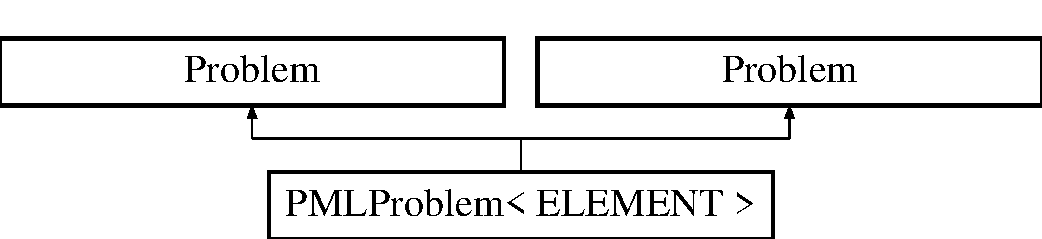
\includegraphics[height=2.000000cm]{classPMLProblem}
\end{center}
\end{figure}
\subsection*{Public Member Functions}
\begin{DoxyCompactItemize}
\item 
\hyperlink{classPMLProblem_ae6cc833e2485ad6d37d6dd14105bf407}{P\+M\+L\+Problem} ()
\begin{DoxyCompactList}\small\item\em Constructor. \end{DoxyCompactList}\item 
\hyperlink{classPMLProblem_a4922fc5b0ef4cf43c41ee9149712adb1}{$\sim$\+P\+M\+L\+Problem} ()
\begin{DoxyCompactList}\small\item\em Destructor (empty) \end{DoxyCompactList}\item 
void \hyperlink{classPMLProblem_a13feb001d09f64dcfe44bbe3c6fe3d97}{actions\+\_\+before\+\_\+newton\+\_\+solve} ()
\begin{DoxyCompactList}\small\item\em Update the problem specs before solve (empty) \end{DoxyCompactList}\item 
void \hyperlink{classPMLProblem_ac171a6a2ff881984b3e057036cbbc414}{actions\+\_\+after\+\_\+newton\+\_\+solve} ()
\begin{DoxyCompactList}\small\item\em Update the problem specs after solve (empty) \end{DoxyCompactList}\item 
void \hyperlink{classPMLProblem_ae04985b020a9e0526ab829ca316adb26}{doc\+\_\+solution} (Doc\+Info \&doc\+\_\+info)
\begin{DoxyCompactList}\small\item\em Doc the solution. Doc\+Info object stores flags/labels for where the output gets written to. \end{DoxyCompactList}\item 
void \hyperlink{classPMLProblem_aa111bfe53d52cf6b2e1bb3b079c16d43}{create\+\_\+pml\+\_\+meshes} ()
\begin{DoxyCompactList}\small\item\em Create P\+ML meshes. \end{DoxyCompactList}\item 
void \hyperlink{classPMLProblem_a2d2cdf5c1e99a7600d91353fd0584d5c}{apply\+\_\+boundary\+\_\+conditions} ()
\begin{DoxyCompactList}\small\item\em Apply boundary conditions. \end{DoxyCompactList}\item 
void \hyperlink{classPMLProblem_a310fb36ad1401d9d975957ecee43accc}{actions\+\_\+before\+\_\+adapt} ()
\begin{DoxyCompactList}\small\item\em Actions before adapt\+: Wipe the P\+ML meshes. \end{DoxyCompactList}\item 
void \hyperlink{classPMLProblem_a732f94d99e7ef65096d6e8d227f9cbc9}{actions\+\_\+after\+\_\+adapt} ()
\begin{DoxyCompactList}\small\item\em Actions after adapt\+: Rebuild the P\+ML meshes. \end{DoxyCompactList}\item 
\hyperlink{classPMLProblem_ae6cc833e2485ad6d37d6dd14105bf407}{P\+M\+L\+Problem} ()
\begin{DoxyCompactList}\small\item\em Constructor. \end{DoxyCompactList}\item 
\hyperlink{classPMLProblem_a4922fc5b0ef4cf43c41ee9149712adb1}{$\sim$\+P\+M\+L\+Problem} ()
\begin{DoxyCompactList}\small\item\em Destructor (empty) \end{DoxyCompactList}\item 
void \hyperlink{classPMLProblem_a13feb001d09f64dcfe44bbe3c6fe3d97}{actions\+\_\+before\+\_\+newton\+\_\+solve} ()
\begin{DoxyCompactList}\small\item\em Update the problem specs before solve (empty) \end{DoxyCompactList}\item 
void \hyperlink{classPMLProblem_ac171a6a2ff881984b3e057036cbbc414}{actions\+\_\+after\+\_\+newton\+\_\+solve} ()
\begin{DoxyCompactList}\small\item\em Update the problem specs after solve (empty) \end{DoxyCompactList}\item 
void \hyperlink{classPMLProblem_ae04985b020a9e0526ab829ca316adb26}{doc\+\_\+solution} (Doc\+Info \&doc\+\_\+info)
\begin{DoxyCompactList}\small\item\em Doc the solution. Doc\+Info object stores flags/labels for where the output gets written to. \end{DoxyCompactList}\item 
void \hyperlink{classPMLProblem_aa111bfe53d52cf6b2e1bb3b079c16d43}{create\+\_\+pml\+\_\+meshes} ()
\begin{DoxyCompactList}\small\item\em Create P\+ML meshes. \end{DoxyCompactList}\item 
void \hyperlink{classPMLProblem_a748701cc016c2bfd07ed2d2467268b5d}{create\+\_\+flux\+\_\+elements} (const unsigned \&b, Mesh $\ast$const \&bulk\+\_\+mesh\+\_\+pt, Mesh $\ast$const \&helmholtz\+\_\+inner\+\_\+boundary\+\_\+mesh\+\_\+pt)
\begin{DoxyCompactList}\small\item\em Create Helmholtz flux elements on boundary b of the Mesh pointed to by bulk\+\_\+mesh\+\_\+pt and add them to the specified surface Mesh. \end{DoxyCompactList}\item 
void \hyperlink{classPMLProblem_afcd6ccc306c79d30d998530c58328b85}{create\+\_\+power\+\_\+elements} (const unsigned \&b, Mesh $\ast$const \&bulk\+\_\+mesh\+\_\+pt, Mesh $\ast$const \&helmholtz\+\_\+power\+\_\+boundary\+\_\+mesh\+\_\+pt)
\begin{DoxyCompactList}\small\item\em Create Helmholtz power elements on boundary b of the Mesh pointed to by bulk\+\_\+mesh\+\_\+pt and add them to the specified surface Mesh. \end{DoxyCompactList}\item 
void \hyperlink{classPMLProblem_a310fb36ad1401d9d975957ecee43accc}{actions\+\_\+before\+\_\+adapt} ()
\begin{DoxyCompactList}\small\item\em Actions before adapt\+: Wipe the P\+ML meshes. \end{DoxyCompactList}\item 
void \hyperlink{classPMLProblem_a732f94d99e7ef65096d6e8d227f9cbc9}{actions\+\_\+after\+\_\+adapt} ()
\begin{DoxyCompactList}\small\item\em Actions after adapt\+: Rebuild the P\+ML meshes. \end{DoxyCompactList}\end{DoxyCompactItemize}
\subsection*{Private Attributes}
\begin{DoxyCompactItemize}
\item 
Refineable\+Triangle\+Mesh$<$ E\+L\+E\+M\+E\+NT $>$ $\ast$ \hyperlink{classPMLProblem_ac8e72d9422ee75522ee98e617dd7e8ae}{Bulk\+\_\+mesh\+\_\+pt}
\begin{DoxyCompactList}\small\item\em Pointer to the refineable \char`\"{}bulk\char`\"{} mesh. \end{DoxyCompactList}\item 
Triangle\+Mesh$<$ E\+L\+E\+M\+E\+NT $>$ $\ast$ \hyperlink{classPMLProblem_a712cffd454213a1eca6d98bd2f0f7e4e}{Bulk\+\_\+mesh\+\_\+pt}
\begin{DoxyCompactList}\small\item\em Pointer to the \char`\"{}bulk\char`\"{} mesh. \end{DoxyCompactList}\item 
Mesh $\ast$ \hyperlink{classPMLProblem_aa325b694fc238fa65549ba5fca9c47ac}{P\+M\+L\+\_\+right\+\_\+mesh\+\_\+pt}
\begin{DoxyCompactList}\small\item\em Pointer to the right P\+ML mesh. \end{DoxyCompactList}\item 
Mesh $\ast$ \hyperlink{classPMLProblem_a94637421e2738f3b6513861a659914e1}{P\+M\+L\+\_\+top\+\_\+mesh\+\_\+pt}
\begin{DoxyCompactList}\small\item\em Pointer to the top P\+ML mesh. \end{DoxyCompactList}\item 
Mesh $\ast$ \hyperlink{classPMLProblem_ab7376c789c76f1150ebbbdf253969136}{P\+M\+L\+\_\+left\+\_\+mesh\+\_\+pt}
\begin{DoxyCompactList}\small\item\em Pointer to the left P\+ML mesh. \end{DoxyCompactList}\item 
Mesh $\ast$ \hyperlink{classPMLProblem_a524a93acb25ace1f12bd1bb4a23d91e3}{P\+M\+L\+\_\+bottom\+\_\+mesh\+\_\+pt}
\begin{DoxyCompactList}\small\item\em Pointer to the bottom P\+ML mesh. \end{DoxyCompactList}\item 
Mesh $\ast$ \hyperlink{classPMLProblem_aa0676946d6e64d7f8eb6174bc12f3b79}{P\+M\+L\+\_\+top\+\_\+right\+\_\+mesh\+\_\+pt}
\begin{DoxyCompactList}\small\item\em Pointer to the top right corner P\+ML mesh. \end{DoxyCompactList}\item 
Mesh $\ast$ \hyperlink{classPMLProblem_aa74e9cdaa9f7d63cd6cd0770e30e2cbe}{P\+M\+L\+\_\+top\+\_\+left\+\_\+mesh\+\_\+pt}
\begin{DoxyCompactList}\small\item\em Pointer to the top left corner P\+ML mesh. \end{DoxyCompactList}\item 
Mesh $\ast$ \hyperlink{classPMLProblem_a51dccc650129c0afd903b4c359a4e6dd}{P\+M\+L\+\_\+bottom\+\_\+right\+\_\+mesh\+\_\+pt}
\begin{DoxyCompactList}\small\item\em Pointer to the bottom right corner P\+ML mesh. \end{DoxyCompactList}\item 
Mesh $\ast$ \hyperlink{classPMLProblem_a0d32b04ee51f2a9e5e14183b212e7815}{P\+M\+L\+\_\+bottom\+\_\+left\+\_\+mesh\+\_\+pt}
\begin{DoxyCompactList}\small\item\em Pointer to the bottom left corner P\+ML mesh. \end{DoxyCompactList}\item 
ofstream \hyperlink{classPMLProblem_a6b343355ccace2851da1860dea7d6a3b}{Trace\+\_\+file}
\begin{DoxyCompactList}\small\item\em Trace file. \end{DoxyCompactList}\item 
Mesh $\ast$ \hyperlink{classPMLProblem_a7aeca36fdbe76a52bb68808f2d4547f2}{Helmholtz\+\_\+inner\+\_\+boundary\+\_\+mesh\+\_\+pt}
\begin{DoxyCompactList}\small\item\em Pointer to the mesh containing the Helmholtz inner boundary condition elements. \end{DoxyCompactList}\item 
Mesh $\ast$ \hyperlink{classPMLProblem_abf7ac369650cc7a876479a208752e02c}{Helmholtz\+\_\+power\+\_\+boundary\+\_\+mesh\+\_\+pt}
\begin{DoxyCompactList}\small\item\em Pointer to mesh of elements that compute the radiated power. \end{DoxyCompactList}\end{DoxyCompactItemize}


\subsection{Detailed Description}
\subsubsection*{template$<$class E\+L\+E\+M\+E\+NT$>$\newline
class P\+M\+L\+Problem$<$ E\+L\+E\+M\+E\+N\+T $>$}

Problem class to demonstrate use of perfectly matched layers for Helmholtz problems. 

Definition at line 79 of file unstructured\+\_\+two\+\_\+d\+\_\+helmholtz.\+cc.



\subsection{Constructor \& Destructor Documentation}
\mbox{\Hypertarget{classPMLProblem_ae6cc833e2485ad6d37d6dd14105bf407}\label{classPMLProblem_ae6cc833e2485ad6d37d6dd14105bf407}} 
\index{P\+M\+L\+Problem@{P\+M\+L\+Problem}!P\+M\+L\+Problem@{P\+M\+L\+Problem}}
\index{P\+M\+L\+Problem@{P\+M\+L\+Problem}!P\+M\+L\+Problem@{P\+M\+L\+Problem}}
\subsubsection{\texorpdfstring{P\+M\+L\+Problem()}{PMLProblem()}\hspace{0.1cm}{\footnotesize\ttfamily [1/2]}}
{\footnotesize\ttfamily template$<$class E\+L\+E\+M\+E\+NT $>$ \\
\hyperlink{classPMLProblem}{P\+M\+L\+Problem}$<$ E\+L\+E\+M\+E\+NT $>$\+::\hyperlink{classPMLProblem}{P\+M\+L\+Problem} (\begin{DoxyParamCaption}{ }\end{DoxyParamCaption})}



Constructor. 

Constructor for Helmholtz problem. 

Definition at line 169 of file unstructured\+\_\+two\+\_\+d\+\_\+helmholtz.\+cc.



References Global\+Parameters\+::\+K\+\_\+squared.

\mbox{\Hypertarget{classPMLProblem_a4922fc5b0ef4cf43c41ee9149712adb1}\label{classPMLProblem_a4922fc5b0ef4cf43c41ee9149712adb1}} 
\index{P\+M\+L\+Problem@{P\+M\+L\+Problem}!````~P\+M\+L\+Problem@{$\sim$\+P\+M\+L\+Problem}}
\index{````~P\+M\+L\+Problem@{$\sim$\+P\+M\+L\+Problem}!P\+M\+L\+Problem@{P\+M\+L\+Problem}}
\subsubsection{\texorpdfstring{$\sim$\+P\+M\+L\+Problem()}{~PMLProblem()}\hspace{0.1cm}{\footnotesize\ttfamily [1/2]}}
{\footnotesize\ttfamily template$<$class E\+L\+E\+M\+E\+NT$>$ \\
\hyperlink{classPMLProblem}{P\+M\+L\+Problem}$<$ E\+L\+E\+M\+E\+NT $>$\+::$\sim$\hyperlink{classPMLProblem}{P\+M\+L\+Problem} (\begin{DoxyParamCaption}{ }\end{DoxyParamCaption})\hspace{0.3cm}{\ttfamily [inline]}}



Destructor (empty) 



Definition at line 88 of file unstructured\+\_\+two\+\_\+d\+\_\+helmholtz.\+cc.

\mbox{\Hypertarget{classPMLProblem_ae6cc833e2485ad6d37d6dd14105bf407}\label{classPMLProblem_ae6cc833e2485ad6d37d6dd14105bf407}} 
\index{P\+M\+L\+Problem@{P\+M\+L\+Problem}!P\+M\+L\+Problem@{P\+M\+L\+Problem}}
\index{P\+M\+L\+Problem@{P\+M\+L\+Problem}!P\+M\+L\+Problem@{P\+M\+L\+Problem}}
\subsubsection{\texorpdfstring{P\+M\+L\+Problem()}{PMLProblem()}\hspace{0.1cm}{\footnotesize\ttfamily [2/2]}}
{\footnotesize\ttfamily template$<$class E\+L\+E\+M\+E\+NT$>$ \\
\hyperlink{classPMLProblem}{P\+M\+L\+Problem}$<$ E\+L\+E\+M\+E\+NT $>$\+::\hyperlink{classPMLProblem}{P\+M\+L\+Problem} (\begin{DoxyParamCaption}{ }\end{DoxyParamCaption})}



Constructor. 

\mbox{\Hypertarget{classPMLProblem_a4922fc5b0ef4cf43c41ee9149712adb1}\label{classPMLProblem_a4922fc5b0ef4cf43c41ee9149712adb1}} 
\index{P\+M\+L\+Problem@{P\+M\+L\+Problem}!````~P\+M\+L\+Problem@{$\sim$\+P\+M\+L\+Problem}}
\index{````~P\+M\+L\+Problem@{$\sim$\+P\+M\+L\+Problem}!P\+M\+L\+Problem@{P\+M\+L\+Problem}}
\subsubsection{\texorpdfstring{$\sim$\+P\+M\+L\+Problem()}{~PMLProblem()}\hspace{0.1cm}{\footnotesize\ttfamily [2/2]}}
{\footnotesize\ttfamily template$<$class E\+L\+E\+M\+E\+NT$>$ \\
\hyperlink{classPMLProblem}{P\+M\+L\+Problem}$<$ E\+L\+E\+M\+E\+NT $>$\+::$\sim$\hyperlink{classPMLProblem}{P\+M\+L\+Problem} (\begin{DoxyParamCaption}{ }\end{DoxyParamCaption})\hspace{0.3cm}{\ttfamily [inline]}}



Destructor (empty) 



Definition at line 260 of file unstructured\+\_\+two\+\_\+d\+\_\+helmholtz\+\_\+scattering.\+cc.



\subsection{Member Function Documentation}
\mbox{\Hypertarget{classPMLProblem_a732f94d99e7ef65096d6e8d227f9cbc9}\label{classPMLProblem_a732f94d99e7ef65096d6e8d227f9cbc9}} 
\index{P\+M\+L\+Problem@{P\+M\+L\+Problem}!actions\+\_\+after\+\_\+adapt@{actions\+\_\+after\+\_\+adapt}}
\index{actions\+\_\+after\+\_\+adapt@{actions\+\_\+after\+\_\+adapt}!P\+M\+L\+Problem@{P\+M\+L\+Problem}}
\subsubsection{\texorpdfstring{actions\+\_\+after\+\_\+adapt()}{actions\_after\_adapt()}\hspace{0.1cm}{\footnotesize\ttfamily [1/2]}}
{\footnotesize\ttfamily template$<$class E\+L\+E\+M\+E\+NT $>$ \\
void \hyperlink{classPMLProblem}{P\+M\+L\+Problem}$<$ E\+L\+E\+M\+E\+NT $>$\+::actions\+\_\+after\+\_\+adapt (\begin{DoxyParamCaption}{ }\end{DoxyParamCaption})}



Actions after adapt\+: Rebuild the P\+ML meshes. 

Actions after adapt\+: Rebuild the face element meshes. 

Definition at line 391 of file unstructured\+\_\+two\+\_\+d\+\_\+helmholtz.\+cc.



References Global\+Parameters\+::\+K\+\_\+squared.

\mbox{\Hypertarget{classPMLProblem_a732f94d99e7ef65096d6e8d227f9cbc9}\label{classPMLProblem_a732f94d99e7ef65096d6e8d227f9cbc9}} 
\index{P\+M\+L\+Problem@{P\+M\+L\+Problem}!actions\+\_\+after\+\_\+adapt@{actions\+\_\+after\+\_\+adapt}}
\index{actions\+\_\+after\+\_\+adapt@{actions\+\_\+after\+\_\+adapt}!P\+M\+L\+Problem@{P\+M\+L\+Problem}}
\subsubsection{\texorpdfstring{actions\+\_\+after\+\_\+adapt()}{actions\_after\_adapt()}\hspace{0.1cm}{\footnotesize\ttfamily [2/2]}}
{\footnotesize\ttfamily template$<$class E\+L\+E\+M\+E\+NT$>$ \\
void \hyperlink{classPMLProblem}{P\+M\+L\+Problem}$<$ E\+L\+E\+M\+E\+NT $>$\+::actions\+\_\+after\+\_\+adapt (\begin{DoxyParamCaption}{ }\end{DoxyParamCaption})}



Actions after adapt\+: Rebuild the P\+ML meshes. 

\mbox{\Hypertarget{classPMLProblem_ac171a6a2ff881984b3e057036cbbc414}\label{classPMLProblem_ac171a6a2ff881984b3e057036cbbc414}} 
\index{P\+M\+L\+Problem@{P\+M\+L\+Problem}!actions\+\_\+after\+\_\+newton\+\_\+solve@{actions\+\_\+after\+\_\+newton\+\_\+solve}}
\index{actions\+\_\+after\+\_\+newton\+\_\+solve@{actions\+\_\+after\+\_\+newton\+\_\+solve}!P\+M\+L\+Problem@{P\+M\+L\+Problem}}
\subsubsection{\texorpdfstring{actions\+\_\+after\+\_\+newton\+\_\+solve()}{actions\_after\_newton\_solve()}\hspace{0.1cm}{\footnotesize\ttfamily [1/2]}}
{\footnotesize\ttfamily template$<$class E\+L\+E\+M\+E\+NT$>$ \\
void \hyperlink{classPMLProblem}{P\+M\+L\+Problem}$<$ E\+L\+E\+M\+E\+NT $>$\+::actions\+\_\+after\+\_\+newton\+\_\+solve (\begin{DoxyParamCaption}{ }\end{DoxyParamCaption})\hspace{0.3cm}{\ttfamily [inline]}}



Update the problem specs after solve (empty) 



Definition at line 94 of file unstructured\+\_\+two\+\_\+d\+\_\+helmholtz.\+cc.

\mbox{\Hypertarget{classPMLProblem_ac171a6a2ff881984b3e057036cbbc414}\label{classPMLProblem_ac171a6a2ff881984b3e057036cbbc414}} 
\index{P\+M\+L\+Problem@{P\+M\+L\+Problem}!actions\+\_\+after\+\_\+newton\+\_\+solve@{actions\+\_\+after\+\_\+newton\+\_\+solve}}
\index{actions\+\_\+after\+\_\+newton\+\_\+solve@{actions\+\_\+after\+\_\+newton\+\_\+solve}!P\+M\+L\+Problem@{P\+M\+L\+Problem}}
\subsubsection{\texorpdfstring{actions\+\_\+after\+\_\+newton\+\_\+solve()}{actions\_after\_newton\_solve()}\hspace{0.1cm}{\footnotesize\ttfamily [2/2]}}
{\footnotesize\ttfamily template$<$class E\+L\+E\+M\+E\+NT$>$ \\
void \hyperlink{classPMLProblem}{P\+M\+L\+Problem}$<$ E\+L\+E\+M\+E\+NT $>$\+::actions\+\_\+after\+\_\+newton\+\_\+solve (\begin{DoxyParamCaption}{ }\end{DoxyParamCaption})\hspace{0.3cm}{\ttfamily [inline]}}



Update the problem specs after solve (empty) 



Definition at line 266 of file unstructured\+\_\+two\+\_\+d\+\_\+helmholtz\+\_\+scattering.\+cc.

\mbox{\Hypertarget{classPMLProblem_a310fb36ad1401d9d975957ecee43accc}\label{classPMLProblem_a310fb36ad1401d9d975957ecee43accc}} 
\index{P\+M\+L\+Problem@{P\+M\+L\+Problem}!actions\+\_\+before\+\_\+adapt@{actions\+\_\+before\+\_\+adapt}}
\index{actions\+\_\+before\+\_\+adapt@{actions\+\_\+before\+\_\+adapt}!P\+M\+L\+Problem@{P\+M\+L\+Problem}}
\subsubsection{\texorpdfstring{actions\+\_\+before\+\_\+adapt()}{actions\_before\_adapt()}\hspace{0.1cm}{\footnotesize\ttfamily [1/2]}}
{\footnotesize\ttfamily template$<$class E\+L\+E\+M\+E\+NT $>$ \\
void \hyperlink{classPMLProblem}{P\+M\+L\+Problem}$<$ E\+L\+E\+M\+E\+NT $>$\+::actions\+\_\+before\+\_\+adapt (\begin{DoxyParamCaption}{ }\end{DoxyParamCaption})}



Actions before adapt\+: Wipe the P\+ML meshes. 

Actions before adapt\+: Wipe the mesh of face elements. 

Definition at line 351 of file unstructured\+\_\+two\+\_\+d\+\_\+helmholtz.\+cc.

\mbox{\Hypertarget{classPMLProblem_a310fb36ad1401d9d975957ecee43accc}\label{classPMLProblem_a310fb36ad1401d9d975957ecee43accc}} 
\index{P\+M\+L\+Problem@{P\+M\+L\+Problem}!actions\+\_\+before\+\_\+adapt@{actions\+\_\+before\+\_\+adapt}}
\index{actions\+\_\+before\+\_\+adapt@{actions\+\_\+before\+\_\+adapt}!P\+M\+L\+Problem@{P\+M\+L\+Problem}}
\subsubsection{\texorpdfstring{actions\+\_\+before\+\_\+adapt()}{actions\_before\_adapt()}\hspace{0.1cm}{\footnotesize\ttfamily [2/2]}}
{\footnotesize\ttfamily template$<$class E\+L\+E\+M\+E\+NT$>$ \\
void \hyperlink{classPMLProblem}{P\+M\+L\+Problem}$<$ E\+L\+E\+M\+E\+NT $>$\+::actions\+\_\+before\+\_\+adapt (\begin{DoxyParamCaption}{ }\end{DoxyParamCaption})}



Actions before adapt\+: Wipe the P\+ML meshes. 

\mbox{\Hypertarget{classPMLProblem_a13feb001d09f64dcfe44bbe3c6fe3d97}\label{classPMLProblem_a13feb001d09f64dcfe44bbe3c6fe3d97}} 
\index{P\+M\+L\+Problem@{P\+M\+L\+Problem}!actions\+\_\+before\+\_\+newton\+\_\+solve@{actions\+\_\+before\+\_\+newton\+\_\+solve}}
\index{actions\+\_\+before\+\_\+newton\+\_\+solve@{actions\+\_\+before\+\_\+newton\+\_\+solve}!P\+M\+L\+Problem@{P\+M\+L\+Problem}}
\subsubsection{\texorpdfstring{actions\+\_\+before\+\_\+newton\+\_\+solve()}{actions\_before\_newton\_solve()}\hspace{0.1cm}{\footnotesize\ttfamily [1/2]}}
{\footnotesize\ttfamily template$<$class E\+L\+E\+M\+E\+NT$>$ \\
void \hyperlink{classPMLProblem}{P\+M\+L\+Problem}$<$ E\+L\+E\+M\+E\+NT $>$\+::actions\+\_\+before\+\_\+newton\+\_\+solve (\begin{DoxyParamCaption}{ }\end{DoxyParamCaption})\hspace{0.3cm}{\ttfamily [inline]}}



Update the problem specs before solve (empty) 



Definition at line 91 of file unstructured\+\_\+two\+\_\+d\+\_\+helmholtz.\+cc.

\mbox{\Hypertarget{classPMLProblem_a13feb001d09f64dcfe44bbe3c6fe3d97}\label{classPMLProblem_a13feb001d09f64dcfe44bbe3c6fe3d97}} 
\index{P\+M\+L\+Problem@{P\+M\+L\+Problem}!actions\+\_\+before\+\_\+newton\+\_\+solve@{actions\+\_\+before\+\_\+newton\+\_\+solve}}
\index{actions\+\_\+before\+\_\+newton\+\_\+solve@{actions\+\_\+before\+\_\+newton\+\_\+solve}!P\+M\+L\+Problem@{P\+M\+L\+Problem}}
\subsubsection{\texorpdfstring{actions\+\_\+before\+\_\+newton\+\_\+solve()}{actions\_before\_newton\_solve()}\hspace{0.1cm}{\footnotesize\ttfamily [2/2]}}
{\footnotesize\ttfamily template$<$class E\+L\+E\+M\+E\+NT$>$ \\
void \hyperlink{classPMLProblem}{P\+M\+L\+Problem}$<$ E\+L\+E\+M\+E\+NT $>$\+::actions\+\_\+before\+\_\+newton\+\_\+solve (\begin{DoxyParamCaption}{ }\end{DoxyParamCaption})\hspace{0.3cm}{\ttfamily [inline]}}



Update the problem specs before solve (empty) 



Definition at line 263 of file unstructured\+\_\+two\+\_\+d\+\_\+helmholtz\+\_\+scattering.\+cc.

\mbox{\Hypertarget{classPMLProblem_a2d2cdf5c1e99a7600d91353fd0584d5c}\label{classPMLProblem_a2d2cdf5c1e99a7600d91353fd0584d5c}} 
\index{P\+M\+L\+Problem@{P\+M\+L\+Problem}!apply\+\_\+boundary\+\_\+conditions@{apply\+\_\+boundary\+\_\+conditions}}
\index{apply\+\_\+boundary\+\_\+conditions@{apply\+\_\+boundary\+\_\+conditions}!P\+M\+L\+Problem@{P\+M\+L\+Problem}}
\subsubsection{\texorpdfstring{apply\+\_\+boundary\+\_\+conditions()}{apply\_boundary\_conditions()}}
{\footnotesize\ttfamily template$<$class E\+L\+E\+M\+E\+NT $>$ \\
void \hyperlink{classPMLProblem}{P\+M\+L\+Problem}$<$ E\+L\+E\+M\+E\+NT $>$\+::apply\+\_\+boundary\+\_\+conditions (\begin{DoxyParamCaption}{ }\end{DoxyParamCaption})}



Apply boundary conditions. 



Definition at line 428 of file unstructured\+\_\+two\+\_\+d\+\_\+helmholtz.\+cc.

\mbox{\Hypertarget{classPMLProblem_a748701cc016c2bfd07ed2d2467268b5d}\label{classPMLProblem_a748701cc016c2bfd07ed2d2467268b5d}} 
\index{P\+M\+L\+Problem@{P\+M\+L\+Problem}!create\+\_\+flux\+\_\+elements@{create\+\_\+flux\+\_\+elements}}
\index{create\+\_\+flux\+\_\+elements@{create\+\_\+flux\+\_\+elements}!P\+M\+L\+Problem@{P\+M\+L\+Problem}}
\subsubsection{\texorpdfstring{create\+\_\+flux\+\_\+elements()}{create\_flux\_elements()}}
{\footnotesize\ttfamily template$<$class E\+L\+E\+M\+E\+NT $>$ \\
void \hyperlink{classPMLProblem}{P\+M\+L\+Problem}$<$ E\+L\+E\+M\+E\+NT $>$\+::create\+\_\+flux\+\_\+elements (\begin{DoxyParamCaption}\item[{const unsigned \&}]{b,  }\item[{Mesh $\ast$const \&}]{bulk\+\_\+mesh\+\_\+pt,  }\item[{Mesh $\ast$const \&}]{helmholtz\+\_\+inner\+\_\+boundary\+\_\+mesh\+\_\+pt }\end{DoxyParamCaption})}



Create Helmholtz flux elements on boundary b of the Mesh pointed to by bulk\+\_\+mesh\+\_\+pt and add them to the specified surface Mesh. 

Create Helmholtz inner Flux Elements on the b-\/th boundary of the Mesh object pointed to by bulk\+\_\+mesh\+\_\+pt and add the elements to the Mesh object pointed to by helmholtz\+\_\+inner\+\_\+boundary\+\_\+mesh\+\_\+pt 

Definition at line 757 of file unstructured\+\_\+two\+\_\+d\+\_\+helmholtz\+\_\+scattering.\+cc.



References P\+M\+L\+Problem$<$ E\+L\+E\+M\+E\+N\+T $>$\+::create\+\_\+power\+\_\+elements(), and Global\+Parameters\+::prescribed\+\_\+incoming\+\_\+flux().

\mbox{\Hypertarget{classPMLProblem_aa111bfe53d52cf6b2e1bb3b079c16d43}\label{classPMLProblem_aa111bfe53d52cf6b2e1bb3b079c16d43}} 
\index{P\+M\+L\+Problem@{P\+M\+L\+Problem}!create\+\_\+pml\+\_\+meshes@{create\+\_\+pml\+\_\+meshes}}
\index{create\+\_\+pml\+\_\+meshes@{create\+\_\+pml\+\_\+meshes}!P\+M\+L\+Problem@{P\+M\+L\+Problem}}
\subsubsection{\texorpdfstring{create\+\_\+pml\+\_\+meshes()}{create\_pml\_meshes()}\hspace{0.1cm}{\footnotesize\ttfamily [1/2]}}
{\footnotesize\ttfamily template$<$class E\+L\+E\+M\+E\+NT $>$ \\
void \hyperlink{classPMLProblem}{P\+M\+L\+Problem}$<$ E\+L\+E\+M\+E\+NT $>$\+::create\+\_\+pml\+\_\+meshes (\begin{DoxyParamCaption}{ }\end{DoxyParamCaption})}



Create P\+ML meshes. 

Create P\+ML meshes and add them to the problem\textquotesingle{}s sub-\/meshes. 

Definition at line 536 of file unstructured\+\_\+two\+\_\+d\+\_\+helmholtz.\+cc.



Referenced by P\+M\+L\+Problem$<$ E\+L\+E\+M\+E\+N\+T $>$\+::create\+\_\+power\+\_\+elements().

\mbox{\Hypertarget{classPMLProblem_aa111bfe53d52cf6b2e1bb3b079c16d43}\label{classPMLProblem_aa111bfe53d52cf6b2e1bb3b079c16d43}} 
\index{P\+M\+L\+Problem@{P\+M\+L\+Problem}!create\+\_\+pml\+\_\+meshes@{create\+\_\+pml\+\_\+meshes}}
\index{create\+\_\+pml\+\_\+meshes@{create\+\_\+pml\+\_\+meshes}!P\+M\+L\+Problem@{P\+M\+L\+Problem}}
\subsubsection{\texorpdfstring{create\+\_\+pml\+\_\+meshes()}{create\_pml\_meshes()}\hspace{0.1cm}{\footnotesize\ttfamily [2/2]}}
{\footnotesize\ttfamily template$<$class E\+L\+E\+M\+E\+NT$>$ \\
void \hyperlink{classPMLProblem}{P\+M\+L\+Problem}$<$ E\+L\+E\+M\+E\+NT $>$\+::create\+\_\+pml\+\_\+meshes (\begin{DoxyParamCaption}{ }\end{DoxyParamCaption})}



Create P\+ML meshes. 

\mbox{\Hypertarget{classPMLProblem_afcd6ccc306c79d30d998530c58328b85}\label{classPMLProblem_afcd6ccc306c79d30d998530c58328b85}} 
\index{P\+M\+L\+Problem@{P\+M\+L\+Problem}!create\+\_\+power\+\_\+elements@{create\+\_\+power\+\_\+elements}}
\index{create\+\_\+power\+\_\+elements@{create\+\_\+power\+\_\+elements}!P\+M\+L\+Problem@{P\+M\+L\+Problem}}
\subsubsection{\texorpdfstring{create\+\_\+power\+\_\+elements()}{create\_power\_elements()}}
{\footnotesize\ttfamily template$<$class E\+L\+E\+M\+E\+NT $>$ \\
void \hyperlink{classPMLProblem}{P\+M\+L\+Problem}$<$ E\+L\+E\+M\+E\+NT $>$\+::create\+\_\+power\+\_\+elements (\begin{DoxyParamCaption}\item[{const unsigned \&}]{b,  }\item[{Mesh $\ast$const \&}]{bulk\+\_\+mesh\+\_\+pt,  }\item[{Mesh $\ast$const \&}]{helmholtz\+\_\+power\+\_\+boundary\+\_\+mesh\+\_\+pt }\end{DoxyParamCaption})}



Create Helmholtz power elements on boundary b of the Mesh pointed to by bulk\+\_\+mesh\+\_\+pt and add them to the specified surface Mesh. 

Create Helmholtz inner Flux Elements on the b-\/th boundary of the Mesh object pointed to by bulk\+\_\+mesh\+\_\+pt and add the elements to the Mesh object pointed to by helmholtz\+\_\+power\+\_\+boundary\+\_\+mesh\+\_\+pt 

Definition at line 793 of file unstructured\+\_\+two\+\_\+d\+\_\+helmholtz\+\_\+scattering.\+cc.



References P\+M\+L\+Problem$<$ E\+L\+E\+M\+E\+N\+T $>$\+::create\+\_\+pml\+\_\+meshes().



Referenced by P\+M\+L\+Problem$<$ E\+L\+E\+M\+E\+N\+T $>$\+::create\+\_\+flux\+\_\+elements().

\mbox{\Hypertarget{classPMLProblem_ae04985b020a9e0526ab829ca316adb26}\label{classPMLProblem_ae04985b020a9e0526ab829ca316adb26}} 
\index{P\+M\+L\+Problem@{P\+M\+L\+Problem}!doc\+\_\+solution@{doc\+\_\+solution}}
\index{doc\+\_\+solution@{doc\+\_\+solution}!P\+M\+L\+Problem@{P\+M\+L\+Problem}}
\subsubsection{\texorpdfstring{doc\+\_\+solution()}{doc\_solution()}\hspace{0.1cm}{\footnotesize\ttfamily [1/2]}}
{\footnotesize\ttfamily template$<$class E\+L\+E\+M\+E\+NT $>$ \\
void \hyperlink{classPMLProblem}{P\+M\+L\+Problem}$<$ E\+L\+E\+M\+E\+NT $>$\+::doc\+\_\+solution (\begin{DoxyParamCaption}\item[{Doc\+Info \&}]{doc\+\_\+info }\end{DoxyParamCaption})}



Doc the solution. Doc\+Info object stores flags/labels for where the output gets written to. 

Doc the solution\+: doc\+\_\+info contains labels/output directory etc. 

Definition at line 459 of file unstructured\+\_\+two\+\_\+d\+\_\+helmholtz.\+cc.



Referenced by main().

\mbox{\Hypertarget{classPMLProblem_ae04985b020a9e0526ab829ca316adb26}\label{classPMLProblem_ae04985b020a9e0526ab829ca316adb26}} 
\index{P\+M\+L\+Problem@{P\+M\+L\+Problem}!doc\+\_\+solution@{doc\+\_\+solution}}
\index{doc\+\_\+solution@{doc\+\_\+solution}!P\+M\+L\+Problem@{P\+M\+L\+Problem}}
\subsubsection{\texorpdfstring{doc\+\_\+solution()}{doc\_solution()}\hspace{0.1cm}{\footnotesize\ttfamily [2/2]}}
{\footnotesize\ttfamily template$<$class E\+L\+E\+M\+E\+NT$>$ \\
void \hyperlink{classPMLProblem}{P\+M\+L\+Problem}$<$ E\+L\+E\+M\+E\+NT $>$\+::doc\+\_\+solution (\begin{DoxyParamCaption}\item[{Doc\+Info \&}]{doc\+\_\+info }\end{DoxyParamCaption})}



Doc the solution. Doc\+Info object stores flags/labels for where the output gets written to. 



\subsection{Member Data Documentation}
\mbox{\Hypertarget{classPMLProblem_ac8e72d9422ee75522ee98e617dd7e8ae}\label{classPMLProblem_ac8e72d9422ee75522ee98e617dd7e8ae}} 
\index{P\+M\+L\+Problem@{P\+M\+L\+Problem}!Bulk\+\_\+mesh\+\_\+pt@{Bulk\+\_\+mesh\+\_\+pt}}
\index{Bulk\+\_\+mesh\+\_\+pt@{Bulk\+\_\+mesh\+\_\+pt}!P\+M\+L\+Problem@{P\+M\+L\+Problem}}
\subsubsection{\texorpdfstring{Bulk\+\_\+mesh\+\_\+pt}{Bulk\_mesh\_pt}\hspace{0.1cm}{\footnotesize\ttfamily [1/2]}}
{\footnotesize\ttfamily template$<$class E\+L\+E\+M\+E\+NT$>$ \\
Triangle\+Mesh$<$ E\+L\+E\+M\+E\+NT $>$ $\ast$ \hyperlink{classPMLProblem}{P\+M\+L\+Problem}$<$ E\+L\+E\+M\+E\+NT $>$\+::Bulk\+\_\+mesh\+\_\+pt\hspace{0.3cm}{\ttfamily [private]}}



Pointer to the refineable \char`\"{}bulk\char`\"{} mesh. 

Pointer to the \char`\"{}bulk\char`\"{} mesh. 

Definition at line 122 of file unstructured\+\_\+two\+\_\+d\+\_\+helmholtz.\+cc.

\mbox{\Hypertarget{classPMLProblem_a712cffd454213a1eca6d98bd2f0f7e4e}\label{classPMLProblem_a712cffd454213a1eca6d98bd2f0f7e4e}} 
\index{P\+M\+L\+Problem@{P\+M\+L\+Problem}!Bulk\+\_\+mesh\+\_\+pt@{Bulk\+\_\+mesh\+\_\+pt}}
\index{Bulk\+\_\+mesh\+\_\+pt@{Bulk\+\_\+mesh\+\_\+pt}!P\+M\+L\+Problem@{P\+M\+L\+Problem}}
\subsubsection{\texorpdfstring{Bulk\+\_\+mesh\+\_\+pt}{Bulk\_mesh\_pt}\hspace{0.1cm}{\footnotesize\ttfamily [2/2]}}
{\footnotesize\ttfamily template$<$class E\+L\+E\+M\+E\+NT$>$ \\
Triangle\+Mesh$<$E\+L\+E\+M\+E\+NT$>$$\ast$ \hyperlink{classPMLProblem}{P\+M\+L\+Problem}$<$ E\+L\+E\+M\+E\+NT $>$\+::Bulk\+\_\+mesh\+\_\+pt\hspace{0.3cm}{\ttfamily [private]}}



Pointer to the \char`\"{}bulk\char`\"{} mesh. 



Definition at line 129 of file unstructured\+\_\+two\+\_\+d\+\_\+helmholtz.\+cc.

\mbox{\Hypertarget{classPMLProblem_a7aeca36fdbe76a52bb68808f2d4547f2}\label{classPMLProblem_a7aeca36fdbe76a52bb68808f2d4547f2}} 
\index{P\+M\+L\+Problem@{P\+M\+L\+Problem}!Helmholtz\+\_\+inner\+\_\+boundary\+\_\+mesh\+\_\+pt@{Helmholtz\+\_\+inner\+\_\+boundary\+\_\+mesh\+\_\+pt}}
\index{Helmholtz\+\_\+inner\+\_\+boundary\+\_\+mesh\+\_\+pt@{Helmholtz\+\_\+inner\+\_\+boundary\+\_\+mesh\+\_\+pt}!P\+M\+L\+Problem@{P\+M\+L\+Problem}}
\subsubsection{\texorpdfstring{Helmholtz\+\_\+inner\+\_\+boundary\+\_\+mesh\+\_\+pt}{Helmholtz\_inner\_boundary\_mesh\_pt}}
{\footnotesize\ttfamily template$<$class E\+L\+E\+M\+E\+NT$>$ \\
Mesh$\ast$ \hyperlink{classPMLProblem}{P\+M\+L\+Problem}$<$ E\+L\+E\+M\+E\+NT $>$\+::Helmholtz\+\_\+inner\+\_\+boundary\+\_\+mesh\+\_\+pt\hspace{0.3cm}{\ttfamily [private]}}



Pointer to the mesh containing the Helmholtz inner boundary condition elements. 



Definition at line 341 of file unstructured\+\_\+two\+\_\+d\+\_\+helmholtz\+\_\+scattering.\+cc.

\mbox{\Hypertarget{classPMLProblem_abf7ac369650cc7a876479a208752e02c}\label{classPMLProblem_abf7ac369650cc7a876479a208752e02c}} 
\index{P\+M\+L\+Problem@{P\+M\+L\+Problem}!Helmholtz\+\_\+power\+\_\+boundary\+\_\+mesh\+\_\+pt@{Helmholtz\+\_\+power\+\_\+boundary\+\_\+mesh\+\_\+pt}}
\index{Helmholtz\+\_\+power\+\_\+boundary\+\_\+mesh\+\_\+pt@{Helmholtz\+\_\+power\+\_\+boundary\+\_\+mesh\+\_\+pt}!P\+M\+L\+Problem@{P\+M\+L\+Problem}}
\subsubsection{\texorpdfstring{Helmholtz\+\_\+power\+\_\+boundary\+\_\+mesh\+\_\+pt}{Helmholtz\_power\_boundary\_mesh\_pt}}
{\footnotesize\ttfamily template$<$class E\+L\+E\+M\+E\+NT$>$ \\
Mesh$\ast$ \hyperlink{classPMLProblem}{P\+M\+L\+Problem}$<$ E\+L\+E\+M\+E\+NT $>$\+::Helmholtz\+\_\+power\+\_\+boundary\+\_\+mesh\+\_\+pt\hspace{0.3cm}{\ttfamily [private]}}



Pointer to mesh of elements that compute the radiated power. 



Definition at line 344 of file unstructured\+\_\+two\+\_\+d\+\_\+helmholtz\+\_\+scattering.\+cc.

\mbox{\Hypertarget{classPMLProblem_a0d32b04ee51f2a9e5e14183b212e7815}\label{classPMLProblem_a0d32b04ee51f2a9e5e14183b212e7815}} 
\index{P\+M\+L\+Problem@{P\+M\+L\+Problem}!P\+M\+L\+\_\+bottom\+\_\+left\+\_\+mesh\+\_\+pt@{P\+M\+L\+\_\+bottom\+\_\+left\+\_\+mesh\+\_\+pt}}
\index{P\+M\+L\+\_\+bottom\+\_\+left\+\_\+mesh\+\_\+pt@{P\+M\+L\+\_\+bottom\+\_\+left\+\_\+mesh\+\_\+pt}!P\+M\+L\+Problem@{P\+M\+L\+Problem}}
\subsubsection{\texorpdfstring{P\+M\+L\+\_\+bottom\+\_\+left\+\_\+mesh\+\_\+pt}{PML\_bottom\_left\_mesh\_pt}}
{\footnotesize\ttfamily template$<$class E\+L\+E\+M\+E\+NT$>$ \\
Mesh $\ast$ \hyperlink{classPMLProblem}{P\+M\+L\+Problem}$<$ E\+L\+E\+M\+E\+NT $>$\+::P\+M\+L\+\_\+bottom\+\_\+left\+\_\+mesh\+\_\+pt\hspace{0.3cm}{\ttfamily [private]}}



Pointer to the bottom left corner P\+ML mesh. 



Definition at line 156 of file unstructured\+\_\+two\+\_\+d\+\_\+helmholtz.\+cc.

\mbox{\Hypertarget{classPMLProblem_a524a93acb25ace1f12bd1bb4a23d91e3}\label{classPMLProblem_a524a93acb25ace1f12bd1bb4a23d91e3}} 
\index{P\+M\+L\+Problem@{P\+M\+L\+Problem}!P\+M\+L\+\_\+bottom\+\_\+mesh\+\_\+pt@{P\+M\+L\+\_\+bottom\+\_\+mesh\+\_\+pt}}
\index{P\+M\+L\+\_\+bottom\+\_\+mesh\+\_\+pt@{P\+M\+L\+\_\+bottom\+\_\+mesh\+\_\+pt}!P\+M\+L\+Problem@{P\+M\+L\+Problem}}
\subsubsection{\texorpdfstring{P\+M\+L\+\_\+bottom\+\_\+mesh\+\_\+pt}{PML\_bottom\_mesh\_pt}}
{\footnotesize\ttfamily template$<$class E\+L\+E\+M\+E\+NT$>$ \\
Mesh $\ast$ \hyperlink{classPMLProblem}{P\+M\+L\+Problem}$<$ E\+L\+E\+M\+E\+NT $>$\+::P\+M\+L\+\_\+bottom\+\_\+mesh\+\_\+pt\hspace{0.3cm}{\ttfamily [private]}}



Pointer to the bottom P\+ML mesh. 



Definition at line 144 of file unstructured\+\_\+two\+\_\+d\+\_\+helmholtz.\+cc.

\mbox{\Hypertarget{classPMLProblem_a51dccc650129c0afd903b4c359a4e6dd}\label{classPMLProblem_a51dccc650129c0afd903b4c359a4e6dd}} 
\index{P\+M\+L\+Problem@{P\+M\+L\+Problem}!P\+M\+L\+\_\+bottom\+\_\+right\+\_\+mesh\+\_\+pt@{P\+M\+L\+\_\+bottom\+\_\+right\+\_\+mesh\+\_\+pt}}
\index{P\+M\+L\+\_\+bottom\+\_\+right\+\_\+mesh\+\_\+pt@{P\+M\+L\+\_\+bottom\+\_\+right\+\_\+mesh\+\_\+pt}!P\+M\+L\+Problem@{P\+M\+L\+Problem}}
\subsubsection{\texorpdfstring{P\+M\+L\+\_\+bottom\+\_\+right\+\_\+mesh\+\_\+pt}{PML\_bottom\_right\_mesh\_pt}}
{\footnotesize\ttfamily template$<$class E\+L\+E\+M\+E\+NT$>$ \\
Mesh $\ast$ \hyperlink{classPMLProblem}{P\+M\+L\+Problem}$<$ E\+L\+E\+M\+E\+NT $>$\+::P\+M\+L\+\_\+bottom\+\_\+right\+\_\+mesh\+\_\+pt\hspace{0.3cm}{\ttfamily [private]}}



Pointer to the bottom right corner P\+ML mesh. 



Definition at line 153 of file unstructured\+\_\+two\+\_\+d\+\_\+helmholtz.\+cc.

\mbox{\Hypertarget{classPMLProblem_ab7376c789c76f1150ebbbdf253969136}\label{classPMLProblem_ab7376c789c76f1150ebbbdf253969136}} 
\index{P\+M\+L\+Problem@{P\+M\+L\+Problem}!P\+M\+L\+\_\+left\+\_\+mesh\+\_\+pt@{P\+M\+L\+\_\+left\+\_\+mesh\+\_\+pt}}
\index{P\+M\+L\+\_\+left\+\_\+mesh\+\_\+pt@{P\+M\+L\+\_\+left\+\_\+mesh\+\_\+pt}!P\+M\+L\+Problem@{P\+M\+L\+Problem}}
\subsubsection{\texorpdfstring{P\+M\+L\+\_\+left\+\_\+mesh\+\_\+pt}{PML\_left\_mesh\_pt}}
{\footnotesize\ttfamily template$<$class E\+L\+E\+M\+E\+NT$>$ \\
Mesh $\ast$ \hyperlink{classPMLProblem}{P\+M\+L\+Problem}$<$ E\+L\+E\+M\+E\+NT $>$\+::P\+M\+L\+\_\+left\+\_\+mesh\+\_\+pt\hspace{0.3cm}{\ttfamily [private]}}



Pointer to the left P\+ML mesh. 



Definition at line 141 of file unstructured\+\_\+two\+\_\+d\+\_\+helmholtz.\+cc.

\mbox{\Hypertarget{classPMLProblem_aa325b694fc238fa65549ba5fca9c47ac}\label{classPMLProblem_aa325b694fc238fa65549ba5fca9c47ac}} 
\index{P\+M\+L\+Problem@{P\+M\+L\+Problem}!P\+M\+L\+\_\+right\+\_\+mesh\+\_\+pt@{P\+M\+L\+\_\+right\+\_\+mesh\+\_\+pt}}
\index{P\+M\+L\+\_\+right\+\_\+mesh\+\_\+pt@{P\+M\+L\+\_\+right\+\_\+mesh\+\_\+pt}!P\+M\+L\+Problem@{P\+M\+L\+Problem}}
\subsubsection{\texorpdfstring{P\+M\+L\+\_\+right\+\_\+mesh\+\_\+pt}{PML\_right\_mesh\_pt}}
{\footnotesize\ttfamily template$<$class E\+L\+E\+M\+E\+NT$>$ \\
Mesh $\ast$ \hyperlink{classPMLProblem}{P\+M\+L\+Problem}$<$ E\+L\+E\+M\+E\+NT $>$\+::P\+M\+L\+\_\+right\+\_\+mesh\+\_\+pt\hspace{0.3cm}{\ttfamily [private]}}



Pointer to the right P\+ML mesh. 



Definition at line 135 of file unstructured\+\_\+two\+\_\+d\+\_\+helmholtz.\+cc.

\mbox{\Hypertarget{classPMLProblem_aa74e9cdaa9f7d63cd6cd0770e30e2cbe}\label{classPMLProblem_aa74e9cdaa9f7d63cd6cd0770e30e2cbe}} 
\index{P\+M\+L\+Problem@{P\+M\+L\+Problem}!P\+M\+L\+\_\+top\+\_\+left\+\_\+mesh\+\_\+pt@{P\+M\+L\+\_\+top\+\_\+left\+\_\+mesh\+\_\+pt}}
\index{P\+M\+L\+\_\+top\+\_\+left\+\_\+mesh\+\_\+pt@{P\+M\+L\+\_\+top\+\_\+left\+\_\+mesh\+\_\+pt}!P\+M\+L\+Problem@{P\+M\+L\+Problem}}
\subsubsection{\texorpdfstring{P\+M\+L\+\_\+top\+\_\+left\+\_\+mesh\+\_\+pt}{PML\_top\_left\_mesh\_pt}}
{\footnotesize\ttfamily template$<$class E\+L\+E\+M\+E\+NT$>$ \\
Mesh $\ast$ \hyperlink{classPMLProblem}{P\+M\+L\+Problem}$<$ E\+L\+E\+M\+E\+NT $>$\+::P\+M\+L\+\_\+top\+\_\+left\+\_\+mesh\+\_\+pt\hspace{0.3cm}{\ttfamily [private]}}



Pointer to the top left corner P\+ML mesh. 



Definition at line 150 of file unstructured\+\_\+two\+\_\+d\+\_\+helmholtz.\+cc.

\mbox{\Hypertarget{classPMLProblem_a94637421e2738f3b6513861a659914e1}\label{classPMLProblem_a94637421e2738f3b6513861a659914e1}} 
\index{P\+M\+L\+Problem@{P\+M\+L\+Problem}!P\+M\+L\+\_\+top\+\_\+mesh\+\_\+pt@{P\+M\+L\+\_\+top\+\_\+mesh\+\_\+pt}}
\index{P\+M\+L\+\_\+top\+\_\+mesh\+\_\+pt@{P\+M\+L\+\_\+top\+\_\+mesh\+\_\+pt}!P\+M\+L\+Problem@{P\+M\+L\+Problem}}
\subsubsection{\texorpdfstring{P\+M\+L\+\_\+top\+\_\+mesh\+\_\+pt}{PML\_top\_mesh\_pt}}
{\footnotesize\ttfamily template$<$class E\+L\+E\+M\+E\+NT$>$ \\
Mesh $\ast$ \hyperlink{classPMLProblem}{P\+M\+L\+Problem}$<$ E\+L\+E\+M\+E\+NT $>$\+::P\+M\+L\+\_\+top\+\_\+mesh\+\_\+pt\hspace{0.3cm}{\ttfamily [private]}}



Pointer to the top P\+ML mesh. 



Definition at line 138 of file unstructured\+\_\+two\+\_\+d\+\_\+helmholtz.\+cc.

\mbox{\Hypertarget{classPMLProblem_aa0676946d6e64d7f8eb6174bc12f3b79}\label{classPMLProblem_aa0676946d6e64d7f8eb6174bc12f3b79}} 
\index{P\+M\+L\+Problem@{P\+M\+L\+Problem}!P\+M\+L\+\_\+top\+\_\+right\+\_\+mesh\+\_\+pt@{P\+M\+L\+\_\+top\+\_\+right\+\_\+mesh\+\_\+pt}}
\index{P\+M\+L\+\_\+top\+\_\+right\+\_\+mesh\+\_\+pt@{P\+M\+L\+\_\+top\+\_\+right\+\_\+mesh\+\_\+pt}!P\+M\+L\+Problem@{P\+M\+L\+Problem}}
\subsubsection{\texorpdfstring{P\+M\+L\+\_\+top\+\_\+right\+\_\+mesh\+\_\+pt}{PML\_top\_right\_mesh\_pt}}
{\footnotesize\ttfamily template$<$class E\+L\+E\+M\+E\+NT$>$ \\
Mesh $\ast$ \hyperlink{classPMLProblem}{P\+M\+L\+Problem}$<$ E\+L\+E\+M\+E\+NT $>$\+::P\+M\+L\+\_\+top\+\_\+right\+\_\+mesh\+\_\+pt\hspace{0.3cm}{\ttfamily [private]}}



Pointer to the top right corner P\+ML mesh. 



Definition at line 147 of file unstructured\+\_\+two\+\_\+d\+\_\+helmholtz.\+cc.

\mbox{\Hypertarget{classPMLProblem_a6b343355ccace2851da1860dea7d6a3b}\label{classPMLProblem_a6b343355ccace2851da1860dea7d6a3b}} 
\index{P\+M\+L\+Problem@{P\+M\+L\+Problem}!Trace\+\_\+file@{Trace\+\_\+file}}
\index{Trace\+\_\+file@{Trace\+\_\+file}!P\+M\+L\+Problem@{P\+M\+L\+Problem}}
\subsubsection{\texorpdfstring{Trace\+\_\+file}{Trace\_file}}
{\footnotesize\ttfamily template$<$class E\+L\+E\+M\+E\+NT$>$ \\
ofstream \hyperlink{classPMLProblem}{P\+M\+L\+Problem}$<$ E\+L\+E\+M\+E\+NT $>$\+::Trace\+\_\+file\hspace{0.3cm}{\ttfamily [private]}}



Trace file. 



Definition at line 159 of file unstructured\+\_\+two\+\_\+d\+\_\+helmholtz.\+cc.



The documentation for this class was generated from the following files\+:\begin{DoxyCompactItemize}
\item 
\hyperlink{unstructured__two__d__helmholtz_8cc}{unstructured\+\_\+two\+\_\+d\+\_\+helmholtz.\+cc}\item 
\hyperlink{unstructured__two__d__helmholtz__scattering_8cc}{unstructured\+\_\+two\+\_\+d\+\_\+helmholtz\+\_\+scattering.\+cc}\end{DoxyCompactItemize}

\hypertarget{classGlobalParameters_1_1TestPMLMapping}{}\section{Global\+Parameters\+:\+:Test\+P\+M\+L\+Mapping Class Reference}
\label{classGlobalParameters_1_1TestPMLMapping}\index{Global\+Parameters\+::\+Test\+P\+M\+L\+Mapping@{Global\+Parameters\+::\+Test\+P\+M\+L\+Mapping}}
Inheritance diagram for Global\+Parameters\+:\+:Test\+P\+M\+L\+Mapping\+:\begin{figure}[H]
\begin{center}
\leavevmode
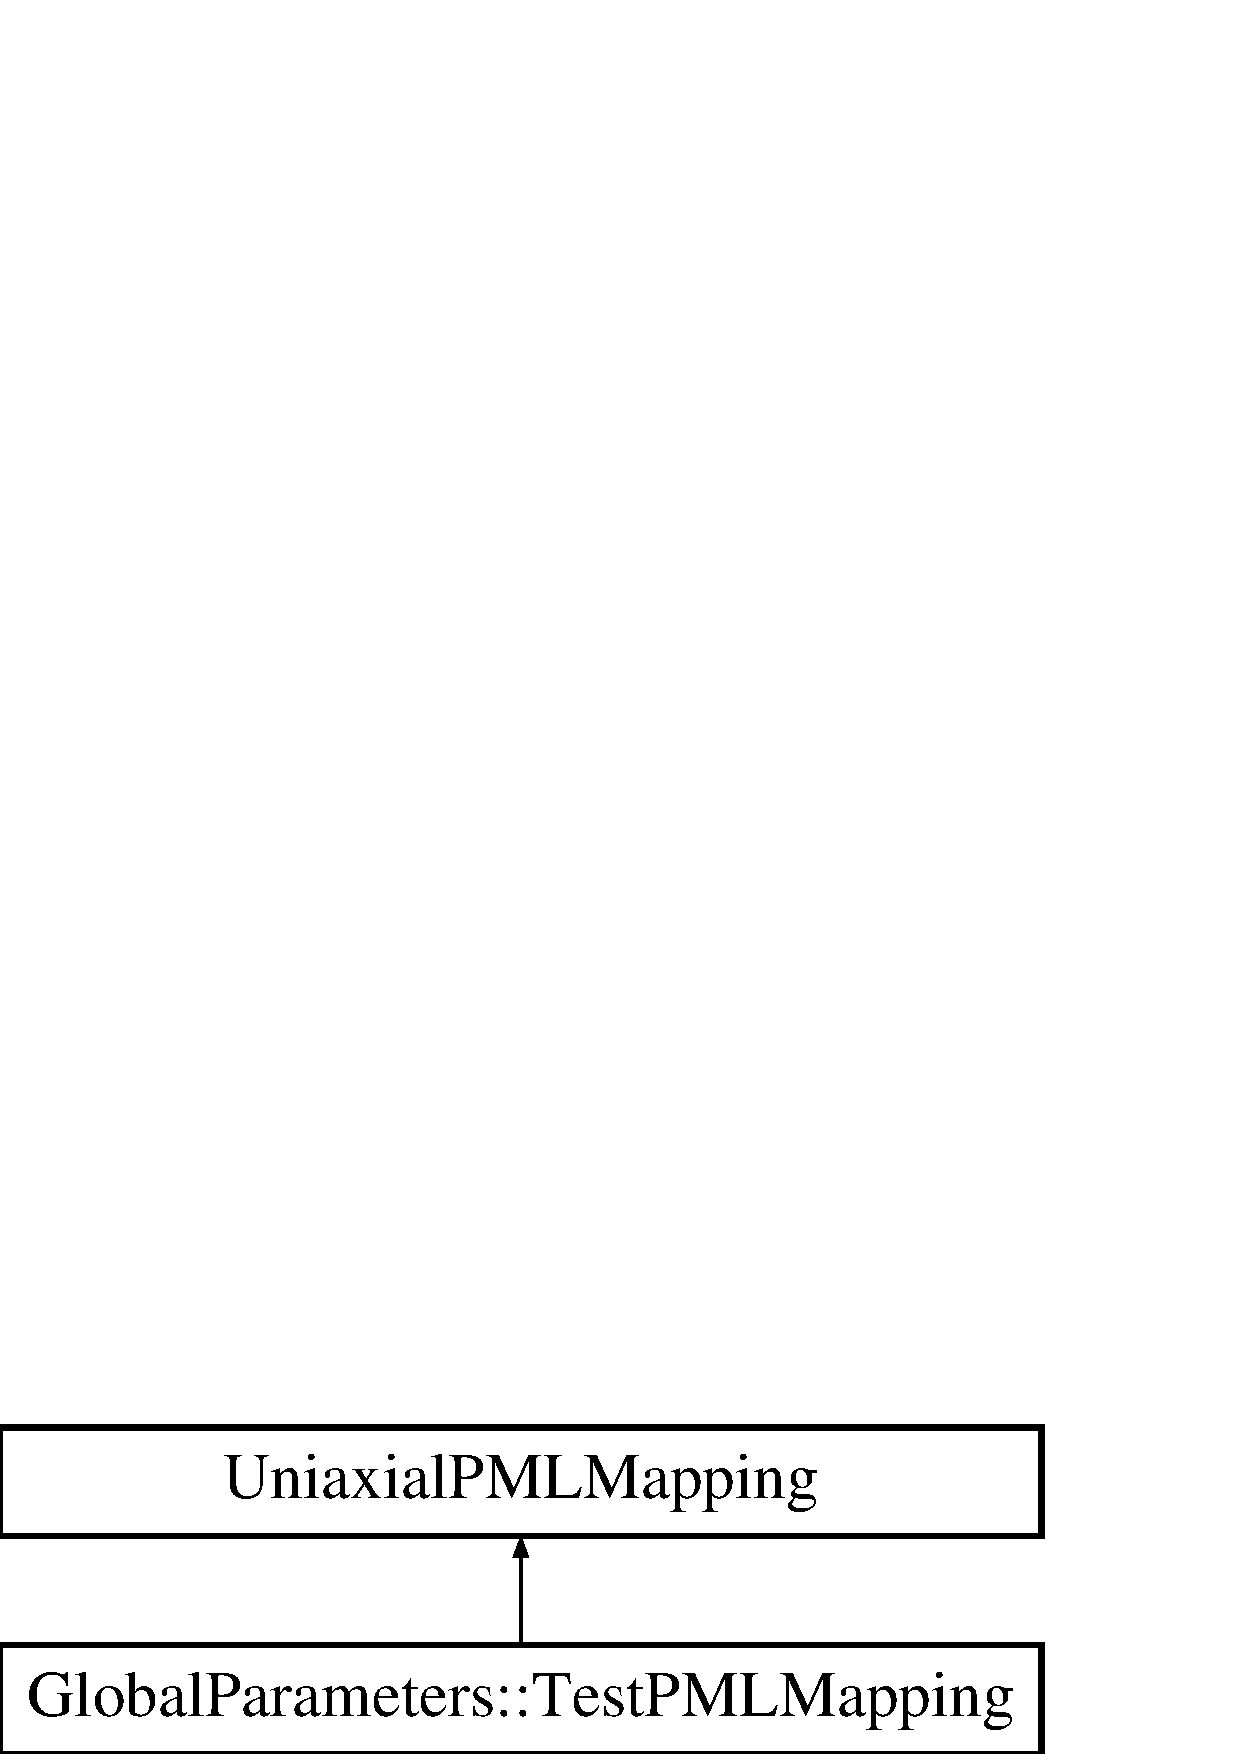
\includegraphics[height=2.000000cm]{classGlobalParameters_1_1TestPMLMapping}
\end{center}
\end{figure}
\subsection*{Public Member Functions}
\begin{DoxyCompactItemize}
\item 
\hyperlink{classGlobalParameters_1_1TestPMLMapping_ac4243d96ef7d60ad7628029a7453480f}{Test\+P\+M\+L\+Mapping} ()
\begin{DoxyCompactList}\small\item\em Default constructor (empty) \end{DoxyCompactList}\item 
std\+::complex$<$ double $>$ \hyperlink{classGlobalParameters_1_1TestPMLMapping_ad3ece98ef692cd1748e1374f7e710514}{dtransformed\+\_\+nu\+\_\+dnu} (const double \&nu, const double \&delta, const double \&wavenumber\+\_\+squared, const double \&alpha\+\_\+shift=0.\+0)
\begin{DoxyCompactList}\small\item\em Overwrite the pure Pml mapping coefficient function to return the coeffcients proposed by Bermudez et al. \end{DoxyCompactList}\item 
std\+::complex$<$ double $>$ \hyperlink{classGlobalParameters_1_1TestPMLMapping_a73188c5c41f61263bebd647f68375732}{transformed\+\_\+nu} (const double \&nu, const double \&delta, const double \&wavenumber\+\_\+squared, const double \&alpha\+\_\+shift=0.\+0)
\end{DoxyCompactItemize}


\subsection{Detailed Description}


Definition at line 206 of file unstructured\+\_\+two\+\_\+d\+\_\+helmholtz\+\_\+scattering.\+cc.



\subsection{Constructor \& Destructor Documentation}
\mbox{\Hypertarget{classGlobalParameters_1_1TestPMLMapping_ac4243d96ef7d60ad7628029a7453480f}\label{classGlobalParameters_1_1TestPMLMapping_ac4243d96ef7d60ad7628029a7453480f}} 
\index{Global\+Parameters\+::\+Test\+P\+M\+L\+Mapping@{Global\+Parameters\+::\+Test\+P\+M\+L\+Mapping}!Test\+P\+M\+L\+Mapping@{Test\+P\+M\+L\+Mapping}}
\index{Test\+P\+M\+L\+Mapping@{Test\+P\+M\+L\+Mapping}!Global\+Parameters\+::\+Test\+P\+M\+L\+Mapping@{Global\+Parameters\+::\+Test\+P\+M\+L\+Mapping}}
\subsubsection{\texorpdfstring{Test\+P\+M\+L\+Mapping()}{TestPMLMapping()}}
{\footnotesize\ttfamily Global\+Parameters\+::\+Test\+P\+M\+L\+Mapping\+::\+Test\+P\+M\+L\+Mapping (\begin{DoxyParamCaption}{ }\end{DoxyParamCaption})\hspace{0.3cm}{\ttfamily [inline]}}



Default constructor (empty) 



Definition at line 212 of file unstructured\+\_\+two\+\_\+d\+\_\+helmholtz\+\_\+scattering.\+cc.



\subsection{Member Function Documentation}
\mbox{\Hypertarget{classGlobalParameters_1_1TestPMLMapping_ad3ece98ef692cd1748e1374f7e710514}\label{classGlobalParameters_1_1TestPMLMapping_ad3ece98ef692cd1748e1374f7e710514}} 
\index{Global\+Parameters\+::\+Test\+P\+M\+L\+Mapping@{Global\+Parameters\+::\+Test\+P\+M\+L\+Mapping}!dtransformed\+\_\+nu\+\_\+dnu@{dtransformed\+\_\+nu\+\_\+dnu}}
\index{dtransformed\+\_\+nu\+\_\+dnu@{dtransformed\+\_\+nu\+\_\+dnu}!Global\+Parameters\+::\+Test\+P\+M\+L\+Mapping@{Global\+Parameters\+::\+Test\+P\+M\+L\+Mapping}}
\subsubsection{\texorpdfstring{dtransformed\+\_\+nu\+\_\+dnu()}{dtransformed\_nu\_dnu()}}
{\footnotesize\ttfamily std\+::complex$<$double$>$ Global\+Parameters\+::\+Test\+P\+M\+L\+Mapping\+::dtransformed\+\_\+nu\+\_\+dnu (\begin{DoxyParamCaption}\item[{const double \&}]{nu,  }\item[{const double \&}]{delta,  }\item[{const double \&}]{wavenumber\+\_\+squared,  }\item[{const double \&}]{alpha\+\_\+shift = {\ttfamily 0.0} }\end{DoxyParamCaption})\hspace{0.3cm}{\ttfamily [inline]}}



Overwrite the pure Pml mapping coefficient function to return the coeffcients proposed by Bermudez et al. 



Definition at line 216 of file unstructured\+\_\+two\+\_\+d\+\_\+helmholtz\+\_\+scattering.\+cc.



References Global\+Parameters\+::\+I().

\mbox{\Hypertarget{classGlobalParameters_1_1TestPMLMapping_a73188c5c41f61263bebd647f68375732}\label{classGlobalParameters_1_1TestPMLMapping_a73188c5c41f61263bebd647f68375732}} 
\index{Global\+Parameters\+::\+Test\+P\+M\+L\+Mapping@{Global\+Parameters\+::\+Test\+P\+M\+L\+Mapping}!transformed\+\_\+nu@{transformed\+\_\+nu}}
\index{transformed\+\_\+nu@{transformed\+\_\+nu}!Global\+Parameters\+::\+Test\+P\+M\+L\+Mapping@{Global\+Parameters\+::\+Test\+P\+M\+L\+Mapping}}
\subsubsection{\texorpdfstring{transformed\+\_\+nu()}{transformed\_nu()}}
{\footnotesize\ttfamily std\+::complex$<$double$>$ Global\+Parameters\+::\+Test\+P\+M\+L\+Mapping\+::transformed\+\_\+nu (\begin{DoxyParamCaption}\item[{const double \&}]{nu,  }\item[{const double \&}]{delta,  }\item[{const double \&}]{wavenumber\+\_\+squared,  }\item[{const double \&}]{alpha\+\_\+shift = {\ttfamily 0.0} }\end{DoxyParamCaption})\hspace{0.3cm}{\ttfamily [inline]}}



Definition at line 226 of file unstructured\+\_\+two\+\_\+d\+\_\+helmholtz\+\_\+scattering.\+cc.



References Global\+Parameters\+::\+I().



The documentation for this class was generated from the following file\+:\begin{DoxyCompactItemize}
\item 
\hyperlink{unstructured__two__d__helmholtz__scattering_8cc}{unstructured\+\_\+two\+\_\+d\+\_\+helmholtz\+\_\+scattering.\+cc}\end{DoxyCompactItemize}

\chapter{File Documentation}
\hypertarget{scattering_8txt__doxygenified_8h}{}\section{scattering.\+txt\+\_\+doxygenified.\+h File Reference}
\label{scattering_8txt__doxygenified_8h}\index{scattering.\+txt\+\_\+doxygenified.\+h@{scattering.\+txt\+\_\+doxygenified.\+h}}

\hypertarget{unstructured__two__d__helmholtz_8cc}{}\section{unstructured\+\_\+two\+\_\+d\+\_\+helmholtz.\+cc File Reference}
\label{unstructured__two__d__helmholtz_8cc}\index{unstructured\+\_\+two\+\_\+d\+\_\+helmholtz.\+cc@{unstructured\+\_\+two\+\_\+d\+\_\+helmholtz.\+cc}}
\subsection*{Classes}
\begin{DoxyCompactItemize}
\item 
class \hyperlink{classPMLProblem}{P\+M\+L\+Problem$<$ E\+L\+E\+M\+E\+N\+T $>$}
\end{DoxyCompactItemize}
\subsection*{Namespaces}
\begin{DoxyCompactItemize}
\item 
 \hyperlink{namespaceGlobalParameters}{Global\+Parameters}
\begin{DoxyCompactList}\small\item\em Namespace for the Helmholtz problem parameters. \end{DoxyCompactList}\end{DoxyCompactItemize}
\subsection*{Functions}
\begin{DoxyCompactItemize}
\item 
int \hyperlink{unstructured__two__d__helmholtz_8cc_a3c04138a5bfe5d72780bb7e82a18e627}{main} (int argc, char $\ast$$\ast$argv)
\begin{DoxyCompactList}\small\item\em Solve 2D Helmholtz problem. \end{DoxyCompactList}\end{DoxyCompactItemize}
\subsection*{Variables}
\begin{DoxyCompactItemize}
\item 
double \hyperlink{namespaceGlobalParameters_a571b847702904d4cf646ac7ff17a7d2c}{Global\+Parameters\+::\+Wavenumber} = sqrt(50.\+0)
\begin{DoxyCompactList}\small\item\em Wavenumber (also known as k), k=omega/c. \end{DoxyCompactList}\item 
double \hyperlink{namespaceGlobalParameters_aae73cb63b27d51a87845c3392cd944eb}{Global\+Parameters\+::\+K\+\_\+squared} = Wavenumber $\ast$ Wavenumber
\begin{DoxyCompactList}\small\item\em Square of the wavenumber (also known as k$^\wedge$2) \end{DoxyCompactList}\end{DoxyCompactItemize}


\subsection{Function Documentation}
\mbox{\Hypertarget{unstructured__two__d__helmholtz_8cc_a3c04138a5bfe5d72780bb7e82a18e627}\label{unstructured__two__d__helmholtz_8cc_a3c04138a5bfe5d72780bb7e82a18e627}} 
\index{unstructured\+\_\+two\+\_\+d\+\_\+helmholtz.\+cc@{unstructured\+\_\+two\+\_\+d\+\_\+helmholtz.\+cc}!main@{main}}
\index{main@{main}!unstructured\+\_\+two\+\_\+d\+\_\+helmholtz.\+cc@{unstructured\+\_\+two\+\_\+d\+\_\+helmholtz.\+cc}}
\subsubsection{\texorpdfstring{main()}{main()}}
{\footnotesize\ttfamily int main (\begin{DoxyParamCaption}\item[{int}]{argc,  }\item[{char $\ast$$\ast$}]{argv }\end{DoxyParamCaption})}



Solve 2D Helmholtz problem. 



Definition at line 637 of file unstructured\+\_\+two\+\_\+d\+\_\+helmholtz.\+cc.



References P\+M\+L\+Problem$<$ E\+L\+E\+M\+E\+N\+T $>$\+::doc\+\_\+solution().


\hypertarget{unstructured__two__d__helmholtz__scattering_8cc}{}\section{unstructured\+\_\+two\+\_\+d\+\_\+helmholtz\+\_\+scattering.\+cc File Reference}
\label{unstructured__two__d__helmholtz__scattering_8cc}\index{unstructured\+\_\+two\+\_\+d\+\_\+helmholtz\+\_\+scattering.\+cc@{unstructured\+\_\+two\+\_\+d\+\_\+helmholtz\+\_\+scattering.\+cc}}
\subsection*{Classes}
\begin{DoxyCompactItemize}
\item 
class \hyperlink{classGlobalParameters_1_1TestPMLMapping}{Global\+Parameters\+::\+Test\+P\+M\+L\+Mapping}
\item 
class \hyperlink{classPMLProblem}{P\+M\+L\+Problem$<$ E\+L\+E\+M\+E\+N\+T $>$}
\end{DoxyCompactItemize}
\subsection*{Namespaces}
\begin{DoxyCompactItemize}
\item 
 \hyperlink{namespaceGlobalParameters}{Global\+Parameters}
\begin{DoxyCompactList}\small\item\em Namespace for the Helmholtz problem parameters. \end{DoxyCompactList}\end{DoxyCompactItemize}
\subsection*{Functions}
\begin{DoxyCompactItemize}
\item 
std\+::complex$<$ double $>$ \hyperlink{namespaceGlobalParameters_a558ef64d34b43c794ef29491cb4840ea}{Global\+Parameters\+::I} (0.\+0, 1.\+0)
\begin{DoxyCompactList}\small\item\em Imaginary unit. \end{DoxyCompactList}\item 
void \hyperlink{namespaceGlobalParameters_ae2320da6053f5527b2af5ebb362a8a07}{Global\+Parameters\+::get\+\_\+exact\+\_\+u} (const Vector$<$ double $>$ \&x, Vector$<$ double $>$ \&u)
\begin{DoxyCompactList}\small\item\em Exact solution for scattered field (vector returns real and impaginary parts). \end{DoxyCompactList}\item 
void \hyperlink{namespaceGlobalParameters_a5183de63b992338ee60bb4da78a45039}{Global\+Parameters\+::prescribed\+\_\+incoming\+\_\+flux} (const Vector$<$ double $>$ \&x, complex$<$ double $>$ \&flux)
\begin{DoxyCompactList}\small\item\em Flux (normal derivative) on the unit disk for a planar incoming wave. \end{DoxyCompactList}\item 
int \hyperlink{unstructured__two__d__helmholtz__scattering_8cc_a3c04138a5bfe5d72780bb7e82a18e627}{main} (int argc, char $\ast$$\ast$argv)
\begin{DoxyCompactList}\small\item\em Solve 2D Helmholtz problem. \end{DoxyCompactList}\end{DoxyCompactItemize}
\subsection*{Variables}
\begin{DoxyCompactItemize}
\item 
unsigned \hyperlink{namespaceGlobalParameters_ae4df03bf0ffa55b741ac846ca7b6c155}{Global\+Parameters\+::\+N\+\_\+fourier} =100
\begin{DoxyCompactList}\small\item\em Number of terms used in the computation of the exact solution. \end{DoxyCompactList}\item 
Test\+P\+M\+L\+Mapping $\ast$ \hyperlink{namespaceGlobalParameters_a66c84b0ba0a324423154d08c56051d0b}{Global\+Parameters\+::\+Test\+\_\+pml\+\_\+mapping\+\_\+pt} = new Test\+P\+M\+L\+Mapping
\end{DoxyCompactItemize}


\subsection{Function Documentation}
\mbox{\Hypertarget{unstructured__two__d__helmholtz__scattering_8cc_a3c04138a5bfe5d72780bb7e82a18e627}\label{unstructured__two__d__helmholtz__scattering_8cc_a3c04138a5bfe5d72780bb7e82a18e627}} 
\index{unstructured\+\_\+two\+\_\+d\+\_\+helmholtz\+\_\+scattering.\+cc@{unstructured\+\_\+two\+\_\+d\+\_\+helmholtz\+\_\+scattering.\+cc}!main@{main}}
\index{main@{main}!unstructured\+\_\+two\+\_\+d\+\_\+helmholtz\+\_\+scattering.\+cc@{unstructured\+\_\+two\+\_\+d\+\_\+helmholtz\+\_\+scattering.\+cc}}
\subsubsection{\texorpdfstring{main()}{main()}}
{\footnotesize\ttfamily int main (\begin{DoxyParamCaption}\item[{int}]{argc,  }\item[{char $\ast$$\ast$}]{argv }\end{DoxyParamCaption})}



Solve 2D Helmholtz problem. 



Definition at line 924 of file unstructured\+\_\+two\+\_\+d\+\_\+helmholtz\+\_\+scattering.\+cc.



References P\+M\+L\+Problem$<$ E\+L\+E\+M\+E\+N\+T $>$\+::doc\+\_\+solution().


%--- End generated contents ---

% Index
\backmatter
\newpage
\phantomsection
\clearemptydoublepage
\addcontentsline{toc}{chapter}{Index}
\printindex

